\documentclass[11pt]{article}
% =====================================================================
%  When Can a Machine Judge Like a Human?
%  Evaluating LLM-as-a-Judge Approaches for Human-Centered Computing Research
%  A three-study CHI paper.  Compile: latexmk -pdf main.tex
% =====================================================================
\usepackage[utf8]{inputenc}
\usepackage[T1]{fontenc}
\usepackage[margin=1in]{geometry}
\usepackage{graphicx}
\graphicspath{{../figures/}}
\usepackage[table,dvipsnames]{xcolor}
\usepackage{booktabs}
\usepackage{longtable}
\usepackage{array}
\usepackage{amsmath,amssymb}
\usepackage{caption}
\usepackage{subcaption}
\usepackage{enumitem}
\usepackage{microtype}
\usepackage[numbers,sort&compress]{natbib}
\usepackage[colorlinks=true,linkcolor=NavyBlue,citecolor=BrickRed,urlcolor=NavyBlue]{hyperref}
\usepackage{titlesec}

\definecolor{g}{RGB}{26,152,80}
\definecolor{a}{RGB}{254,224,139}
\definecolor{r}{RGB}{215,48,39}
\newcommand{\corpustabref}{Table~\ref{tab:full}}          % full Study-1a corpus (appendix here)
\newcommand{\sttwotabref}{Table~\ref{tab:study2full}}     % full Study-2 corpus (appendix here)

% auto-generated - do not edit by hand (see analysis/make_figures.py)
\newcommand{\Nstudies}{217}
\newcommand{\Ndomains}{29}
\newcommand{\Nvalidated}{8}
\newcommand{\Npromising}{60}
\newcommand{\Nmixed}{108}
\newcommand{\Ncaution}{39}
\newcommand{\Nunreliable}{2}
\newcommand{\Pctreliable}{31}
\newcommand{\Pctproblematic}{19}
\newcommand{\Nnumeric}{29}
\newcommand{\Nprimary}{206}
\newcommand{\Nsecondary}{11}
\newcommand{\Ngreen}{8}
\newcommand{\Namber}{19}
\newcommand{\Nred}{2}
\newcommand{\OAretrieved}{1500}
\newcommand{\OAunique}{957}
\newcommand{\OAtopical}{165}
\newcommand{\Webhits}{472}
\newcommand{\Webunique}{304}
\newcommand{\Nassessed}{263}
\newcommand{\Nexclscreen}{967}
\newcommand{\Crossdup}{31}
\newcommand{\Meanrel}{3.15}
\newcommand{\Nparity}{15}
        % Study 1 macros (\Nstudies, \Ndomains, ...)
% auto-generated
\newcommand{\STN}{55}
\newcommand{\STaugment}{36}
\newcommand{\STreplace}{14}
\newcommand{\STsimulate}{5}
\newcommand{\STtension}{38}
\newcommand{\STcritical}{8}
\newcommand{\STenabling}{9}
\newcommand{\SThci}{22}
\newcommand{\STmethods}{15}
\newcommand{\STrelaugment}{3.17}
\newcommand{\STrelreplace}{3.07}
\newcommand{\STrelsim}{2.8}
\newcommand{\STincluded}{55}
\newcommand{\SToa}{857}
 % Study 2 macros (\STN, \STaugment, ...)
% auto-generated
\newcommand{\STHRn}{15000}
\newcommand{\STHRdatasets}{5}
\newcommand{\STHRmodels}{6}
\newcommand{\STHRpass}{6}
 % Study 3 macros (\STHRn, \STHRdatasets, ...)
% auto-generated by results_table1b.py
\newcommand{\ONEmodels}{4}
\newcommand{\ONEpanel}{\texttt{deepseek-v4-pro}, \texttt{glm-5.1}, \texttt{gptoss-120b}, \texttt{qwen3.6-35b-a3b}}
\newcommand{\ONEnjudg}{25,600}
\newcommand{\ONEbest}{\texttt{deepseek-v4-pro}}
\newcommand{\ONEbestrho}{0.542}
\newcommand{\ONEreportedrho}{0.52}
\newcommand{\ONEbeataspects}{1}
\newcommand{\ONEnsurpass}{3}
\newcommand{\ONEverdictphrase}{The most powerful open models now \emph{match or exceed} the reported proprietary-judge correlations on SummEval.}
      % Study 1b macros (\ONEbest, \ONEbestrho, ...)
% auto-generated by mixed_effects.py
\newcommand{\SMEsubjOR}{0.21}
\newcommand{\SMEsubjP}{6e-6}
\newcommand{\SMEsizeOR}{1.22}
\newcommand{\SMEsizeP}{0.000}
\newcommand{\SMEsizeZ}{9.63}
\newcommand{\SMEfdrtests}{30}
\newcommand{\SMEfdrsig}{25}
\newcommand{\SMEfdrbelow}{20}
\newcommand{\SMEfdrabove}{5}
\newcommand{\SMEvcdataset}{0.83}
\newcommand{\SMEvcitem}{2.21}
\newcommand{\SMEglmmsubj}{-0.57}
\newcommand{\SMEglmmsize}{0.37}
 % Study 3 inferential macros (\SMEsubjOR, \SMEfdrsig, ...)

\titleformat{\section}{\large\bfseries}{\thesection}{0.6em}{}
\titleformat{\subsection}{\normalsize\bfseries}{\thesubsection}{0.6em}{}

\title{\textbf{When Can a Machine Judge Like a Human?}\\[3pt]
\large Evaluating LLM-as-a-Judge Approaches for Human-Centered Computing Research}
\author{Carlos Toxtli\thanks{Correspondence: \texttt{ai4helab@gmail.com}. This research used an AI-assisted
systematic-search and extraction pipeline; all search logs (OpenAlex, Semantic Scholar, web), the two extracted
study corpora, the analysis code, the figure/table-generation scripts, and the Study-3 evaluation harness are
released for full reproducibility.}}
\date{May 2026}

\begin{document}
\maketitle

\begin{abstract}
\noindent
Large language models (LLMs) are flooding into Human-Centered Computing (HCC) research as substitutes for human
judgment: coding qualitative data, annotating crowdsourced corpora, simulating study participants, generating
personas, and evaluating designs. Yet HCC's methods carry epistemological commitments (interpretation, reflexivity,
positionality) that make uncritical substitution risky, and the field lacks an evidence-based account of
\emph{when} an ``LLM-as-a-judge'' can stand in for a human and when it cannot. We address this with four studies.
\textbf{Study 1a} is a PRISMA systematic review of \Nstudies{} studies across \Ndomains{} domains that establishes
the general reliability landscape of LLM-as-a-judge: substitution is validated ($\approx$ or above the
human-human ceiling) for objective, verifiable, low-expertise tasks judged in aggregate, and unreliable for
subjective, expert, low-resource, or adversarial ones (mean reliability \Meanrel/5; only \Pctreliable\% of studies
in the reliable band). \textbf{Study 1b} asks whether this landscape is a moving target: we re-run a flagship
``promising'' benchmark (SummEval) with the most powerful open models served via Clemson's vLLM API and ask whether
they now \emph{surpass} the agreement numbers reported for proprietary judges, distinguishing a ``matter of time''
from a structural ceiling. \textbf{Study 2} is a PRISMA systematic review of \STN{} studies focused on HCC, HCI, and
qualitative-research methods that historically require human input. It finds that the field overwhelmingly positions
LLMs to \emph{augment} rather than replace humans (\STaugment{} augment vs.\ \STreplace{} replace vs.\ \STsimulate{}
simulate), with an epistemic stance dominated by \emph{tension} (\STtension/\STN); objective crowd-annotation
substitution is validated, interpretive qualitative analysis is reliable only as human-in-the-loop augmentation, and
\emph{simulating} participants, personas, and usability evaluations is the least reliable (flattening of identity
groups, caricature, hallucinated usability issues). \textbf{Study 3} closes the gaps the
first two studies expose, by running a standardized LLM-as-a-judge meta-evaluation, using open models served via
Clemson's vLLM API and the agreement-against-human-ceiling methodology distilled from Studies 1-2, on HCC datasets
that contain human labels but have never been formally tested with an LLM judge. Across \STHRn{} judgments (a
6-model open panel, 9B-754B), it finds the human-agreement ceiling governs reliability: the panel matches or
exceeds humans on low-ceiling NLI but falls short of, and fails the alt-test for, subjective social-computing
annotation (emotion, hate speech), with binary offensiveness the strongest case. A mixed-effects model confirms the
mechanism: judge correctness is governed overwhelmingly by item-level human (dis)agreement (random-intercept
$\mathrm{SD}_{\text{item}}=\SMEvcitem$) and by task subjectivity ($\mathrm{OR}=\SMEsubjOR$ per unit of
$1\!-\!$ceiling), while model scale contributes only modestly ($\mathrm{OR}=\SMEsizeOR$ per $\log_{10}$ params);
after FDR correction \SMEfdrbelow{} of \SMEfdrtests{} judge$\times$dataset cells sit significantly below the human
ceiling. Together the studies yield a
decision framework telling HCC researchers when an LLM judge is a validated substitute, a human-in-the-loop
assistant, or an unsafe replacement.

\end{abstract}

\tableofcontents
\bigskip

\section{Introduction and motivation}
% =====================================================================
In barely two years, LLMs have moved from objects of HCI study to \emph{instruments} of HCI method. Researchers now
use them to code interview transcripts \citep{xiao2023support,gao2024collabcoder}, run thematic analyses
\citep{depaoli2023inductive,dai2023llminloop}, annotate social-media corpora \citep{gilardi2023chatgpt,
tornberg2023political}, simulate survey respondents and ``silicon samples'' \citep{argyle2023outofone}, generate
personas \citep{salminen2024deusexmachina}, and even perform heuristic usability evaluation \citep{guerino2025gpt4ousability}.
The appeal is obvious: human judgment is the costly bottleneck of human-centered research, and an LLM that labels for
\$0.003 an item is a tempting stand-in \citep{gilardi2023chatgpt}.

The danger is equally clear. HCC and qualitative methods are not mere labeling pipelines; they carry
\emph{epistemological commitments} (interpretation, reflexivity, positionality, and the situated knowledge of the
researcher) that an LLM cannot obviously honor \citep{schroeder2025usestensions,davison2024ethics}. Substituting a
model for a human participant can \emph{flatten} and misportray the very identity groups HCI seeks to center
\citep{wang2024flatten,cheng2023compost}. And the empirical record is genuinely mixed: the same model can match two
human coders on a structured codebook \citep{dunivin2024scalablecot} yet hallucinate usability problems that do not
exist \citep{guerino2025gpt4ousability}, or agree with a second annotator on stance \citep{gilardi2023chatgpt} yet be
fooled into mislabeling relevance by a few injected keywords \citep{alaofi2024fooledrelevant}.

HCC researchers therefore face a question with no consolidated answer: \textbf{for which HCC research tasks is an
LLM-as-a-judge a safe substitute for human judgment, for which is it a useful assistant, and for which is it
unsafe?} This paper answers that question through three studies with a deliberate progression
(Figure~\ref{fig:overview}):

\begin{enumerate}[leftmargin=1.5em,itemsep=2pt]
\item \textbf{Study 1a, the general landscape.} A PRISMA systematic review of \Nstudies{} studies across
\Ndomains{} domains establishes \emph{where, in general}, LLM-as-a-judge agrees with humans, anchored to the
human-human ceiling. This gives HCC the broad map and the methodological vocabulary (the reliability rubric, the
bias catalogue, the decision map).
\item \textbf{Study 1b, is the landscape a moving target?} The review captures results \emph{as reported}, often
with one- or two-generation-old proprietary judges. We re-run a flagship ``promising''-band benchmark (SummEval
summarization quality) with the \emph{most powerful open models available today} and ask whether they now surpass
the canonical reported judge correlations, separating limitations that are a ``matter of time'' (scale/recency)
from \emph{structural} ceilings that more capable models do not cross.
\item \textbf{Study 2, the HCC lens.} A second PRISMA review of \STN{} studies zooms into the methods HCC
actually uses (qualitative coding, thematic/content analysis, crowdsourced annotation, participant simulation,
persona generation, usability evaluation, and design critique) and codes how the field positions LLMs (augment /
replace / simulate) and with what epistemic stance.
\item \textbf{Study 3, filling the gaps.} Studies 1-2 reveal HCC datasets that contain human labels
but have never been formally evaluated with an LLM judge. Study 3 runs a standardized LLM-as-a-judge
meta-evaluation on these datasets, using open models served through \PROVIDER{} and the
agreement-against-human-ceiling methodology distilled from the prior literature, with a mixed-effects analysis of
what governs judge reliability.
\end{enumerate}

\begin{figure}[t]\centering
\fbox{\parbox{0.96\linewidth}{\centering\small
\textbf{Study 1a}: \emph{Where} is LLM-as-a-judge reliable? (cross-domain review, \Nstudies{} studies)
\;$\rightarrow$\;
\textbf{Study 1b}: \emph{Is it a moving target?} (most powerful open models vs reported numbers, SummEval)
\;$\rightarrow$\;
\textbf{Study 2}: \emph{How does HCC use LLMs} for human-input tasks? (\STN{} studies)
\;$\rightarrow$\;
\textbf{Study 3}: \emph{Fill the gaps}, standardized evaluation on HCC datasets with human labels (open models via
\PROVIDER{}).}}
\caption{The four-study progression. Study~1a maps where LLM judges are reliable; Study~1b tests whether today's
strongest open models move that map; Study~2 narrows to Human-Centered Computing practice; Study~3 supplies new
empirical evidence on under-tested HCC datasets.}
\label{fig:overview}
\end{figure}

\paragraph{Contributions.} (1) The first consolidated, human-ceiling-anchored map of LLM-as-a-judge reliability
across \Ndomains{} domains (Study 1a). (2) A direct test of whether the most powerful open models available today
surpass the reported judge correlations in a flagship ``promising'' domain, adjudicating ``matter of time'' vs.\
structural ceiling (Study 1b). (3) The first systematic review of LLM substitution \emph{specifically} for
HCC/HCI/qualitative methods, with a method$\times$role$\times$stance coding that surfaces the field's
augment-not-replace consensus and its epistemic tensions (Study 2). (4) A reproducible, standardized evaluation
harness plus a mixed-effects account of what governs judge reliability (Study 3), tested on HCC datasets that had
human labels but no prior LLM-judge evaluation, plus two released corpora ($\Nstudies+\STN$ coded studies), all
code, and a decision framework for practitioners.

% =====================================================================
\section{Background and shared methodology}
% =====================================================================
LLM-as-a-judge descends from reference-free metrics (BERTScore, COMET) but uses a general instruction-following
model with a natural-language rubric, supporting pointwise, pairwise, and listwise judgment
\citep{li2024compsurvey,gu2024survey}. Four architectural families recur: prompted general LLMs
\citep{zheng2023mtbench,liu2023geval}; fine-tuned open evaluators \citep{kim2023prometheus,zhu2023judgelm,
wang2023pandalm}; juries/multi-agent panels \citep{verga2024poll,chan2023chateval}; and calibrated rubric methods
\citep{hashemi2024llmrubric}. Prior surveys taxonomize methodology \citep{gu2024survey,li2024gen2judge}; we instead
synthesize \emph{where substitution is empirically validated}, and, uniquely, do so through the HCC lens.

\paragraph{Related work.} Four literatures meet in this paper. (1) \emph{LLM-as-a-judge evaluation}: studies report
strong agreement on aggregate, verifiable tasks (MT-Bench \citep{zheng2023mtbench}, GEMBA \citep{kocmi2023gembamqm},
SAFE factuality \citep{wei2024safe}) but document systematic biases (position, verbosity, self-preference, and an
expertise gap by which judges converge on crowd rather than expert consensus \citep{bavaresco2024judgebench}), which
motivates benchmarking against the human ceiling rather than against a single ``gold.'' (2) \emph{LLMs in HCI and
qualitative research}: a fast-growing body uses LLMs to assist coding and thematic analysis
\citep{xiao2023support,gao2024collabcoder,dai2023llminloop} while qualitative scholars warn that interpretation,
reflexivity, and positionality resist automation \citep{schroeder2025usestensions,davison2024ethics}. (3)
\emph{Participant and persona simulation}: ``silicon samples'' \citep{argyle2023outofone} and synthetic users are
increasingly scrutinized for flattening identity and distorting variance
\citep{wang2024flatten,cheng2023compost,bisbee2023perils}. (4) \emph{Learning with disagreement and perspectivism}:
work on annotator disagreement and human label variation \citep{calderon2025alttest} argues that for subjective
constructs the ``ceiling'' is itself low and contested, which our Study 3 datasets (ChaosNLI, GoEmotions, MultiPICo)
operationalize directly. We connect these threads with two methodological commitments often missing from
judge evaluations: anchoring every verdict to the \emph{human-human} ceiling, and probing \emph{data contamination}
so that agreement on older public datasets is not mistaken for genuine competence.

\paragraph{Shared protocol.} Both reviews follow PRISMA~2020 \citep{page2021prisma}, identify studies through a
triangulated search (the OpenAlex API as the primary bibliographic database, Semantic Scholar as a cross-check, and
a structured web ``deep-research'' arm), and code each study on a five-level \textbf{reliability verdict}
benchmarked against the \emph{human-human agreement ceiling} for the same task: \textbf{1 Validated}
($\approx$/$>$ ceiling), \textbf{2 Promising} (conditional), \textbf{3 Mixed} (task-dependent), \textbf{4 Caution}
(below ceiling), \textbf{5 Unreliable} (near chance / bias-dominated). We report a reliability score $=6-$verdict
and synthesize within metric families rather than pooling incommensurable effect sizes. Full protocols, search
logs, and the two coded corpora are released.

% =====================================================================
\section{Study 1a: The cross-domain reliability landscape}
% =====================================================================
\subsection{Method (summary)}
Study 1a systematically reviewed \Nstudies{} studies across \Ndomains{} domains comparing LLM-as-a-judge to human
annotation. Identification triangulated OpenAlex (\OAretrieved{} records, \OAunique{} unique), Semantic Scholar, and
a 59-query web search; screening retained on-topic empirical comparisons; \Nnumeric{} studies reported an
extractable numeric agreement value (Figure~\ref{fig:prisma1}; the full coded corpus is \corpustabref).

\begin{figure}[t]\centering
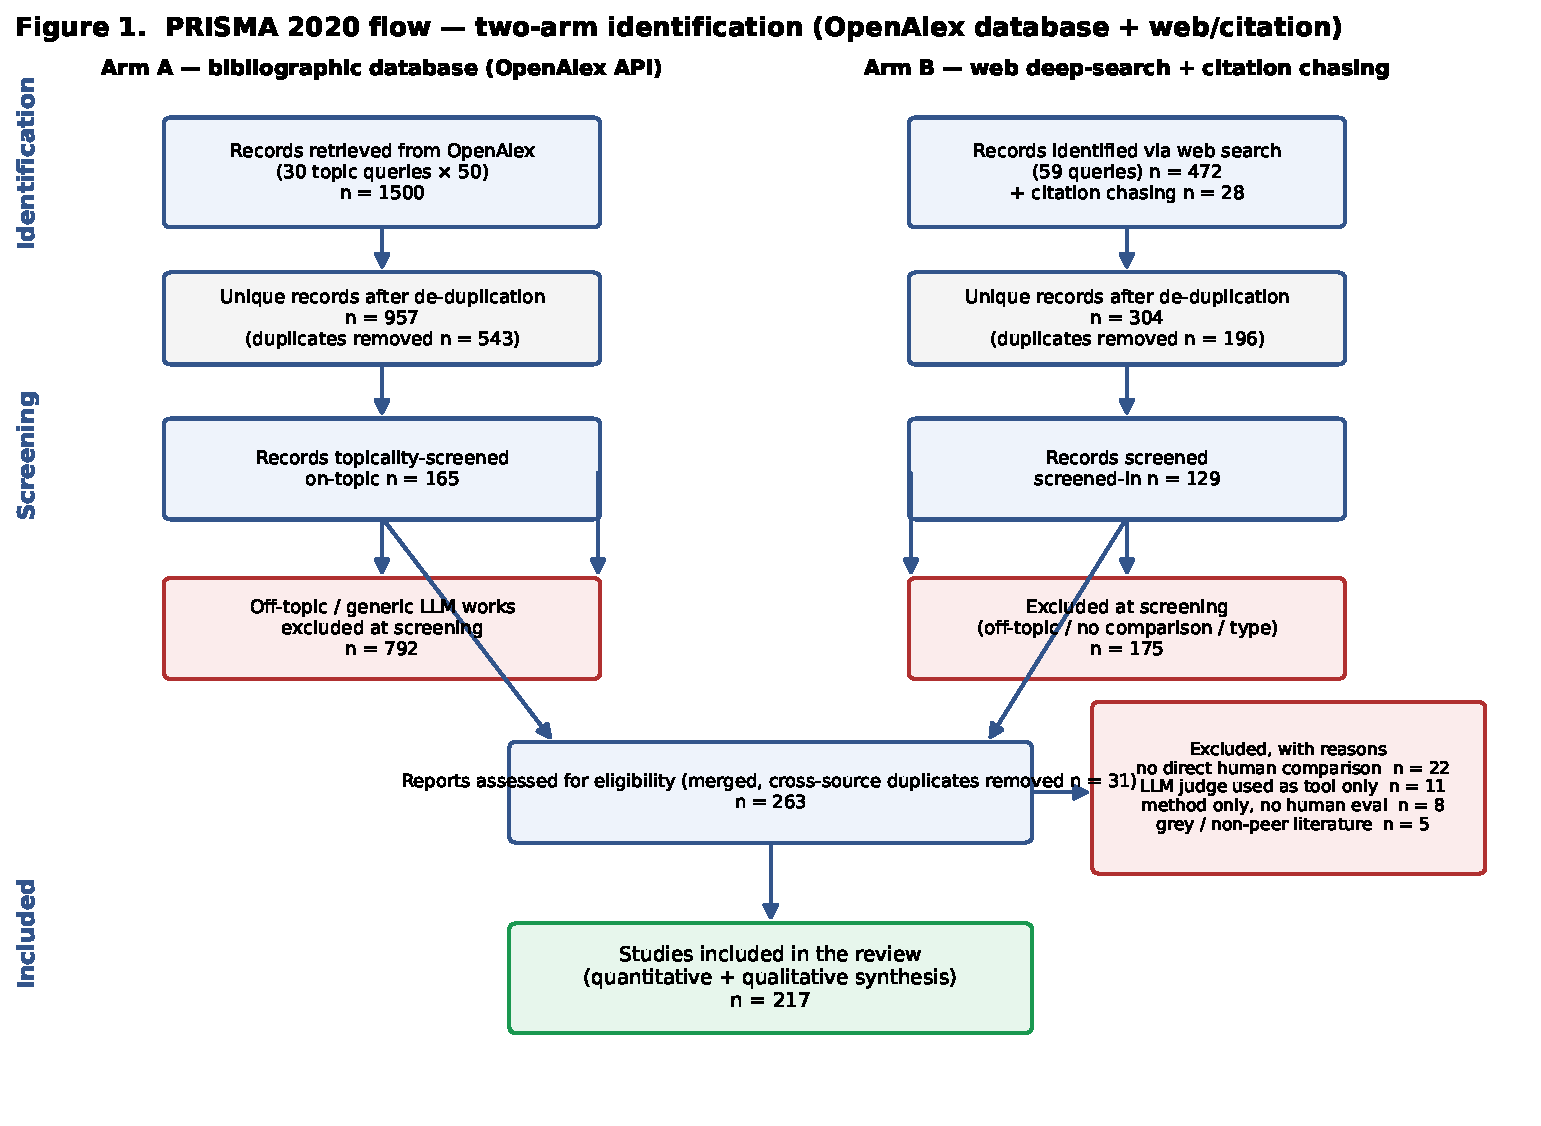
\includegraphics[width=0.96\linewidth]{fig01_prisma_flow}
\caption{Study 1a PRISMA~2020 flow (two-arm identification: OpenAlex database + web/citation).}
\label{fig:prisma1}
\end{figure}

\subsection{Findings: a green/amber/red landscape}
The modal verdict is \emph{mixed/task-dependent}; only \Pctreliable\% of studies sit in the reliable band and
\Pctproblematic\% in the problematic band (mean reliability \Meanrel/5). Reliability is governed by three properties:
\textbf{objectivity}, \textbf{tractable verification}, and a \textbf{low human-agreement floor}.
\textbf{Green ($\ge$3.5; \Ngreen{} domains):} machine translation (system level), text-to-image alignment,
verifiable instruction-following, QA/factuality, information extraction, general-NLG pairwise preference, dialogue,
and legal scoring: here LLM judges frequently match or exceed the human ceiling (e.g., MT-Bench 85\% vs.\ 81\%
human-human \citep{zheng2023mtbench}; GEMBA-MQM 96.5\% \citep{kocmi2023gembamqm}; SAFE wins 76\% of disagreements
\citep{wei2024safe}). \textbf{Amber (\Namber{} domains):} summarization, RAG, education, social-science annotation,
medicine (structure-dependent: $\kappa\!\approx\!0.82$-$0.93$ structured vs.\ $0.47$-$0.71$ complex reasoning),
code, and IR/relevance (strong but contested \citep{clarke2024cantreplace}). \textbf{Red (\Nred{} domains):}
low-resource multilingual evaluation and creative writing (near-zero expert correlation
\citep{chakrabarty2024artartifice}). Figures~\ref{fig:dom1}-\ref{fig:land1} give the domain ordering and the
domain$\times$task landscape; the decision map (Figure~\ref{fig:dec1}) positions domains by reliability against
stakes.

\begin{figure}[t]\centering
\begin{subfigure}{0.5\linewidth}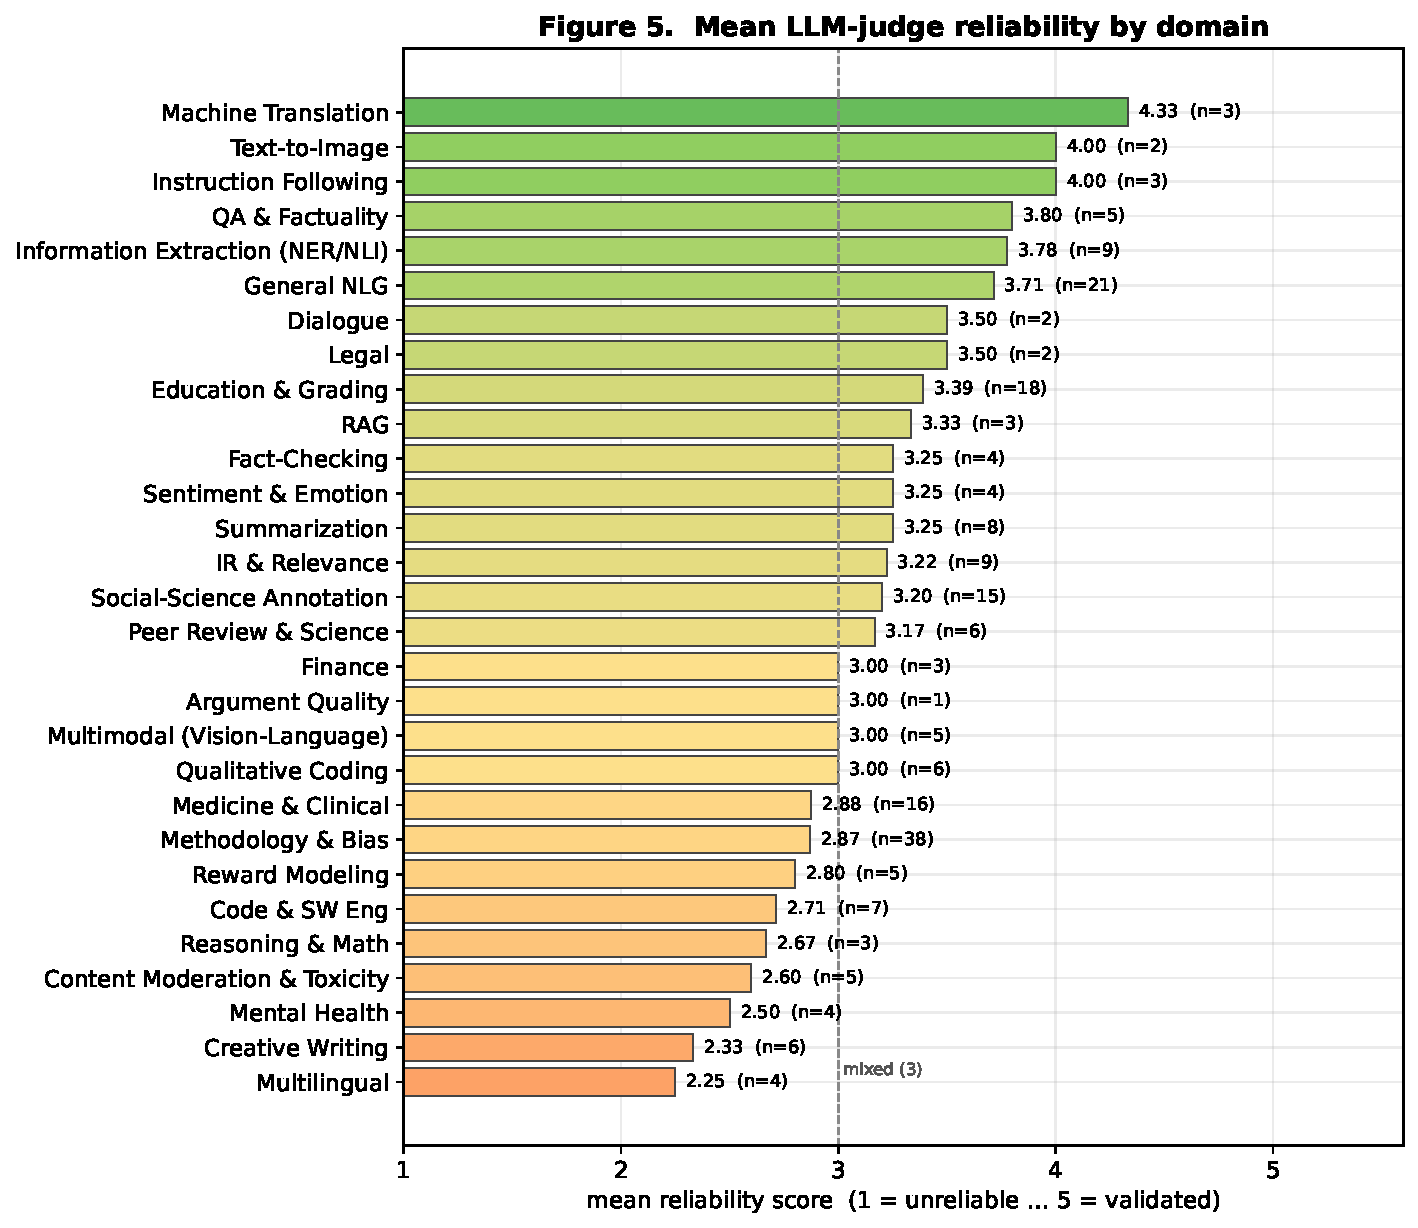
\includegraphics[width=\linewidth]{fig05_reliability_by_domain}\caption{}\label{fig:dom1}\end{subfigure}\hfill
\begin{subfigure}{0.48\linewidth}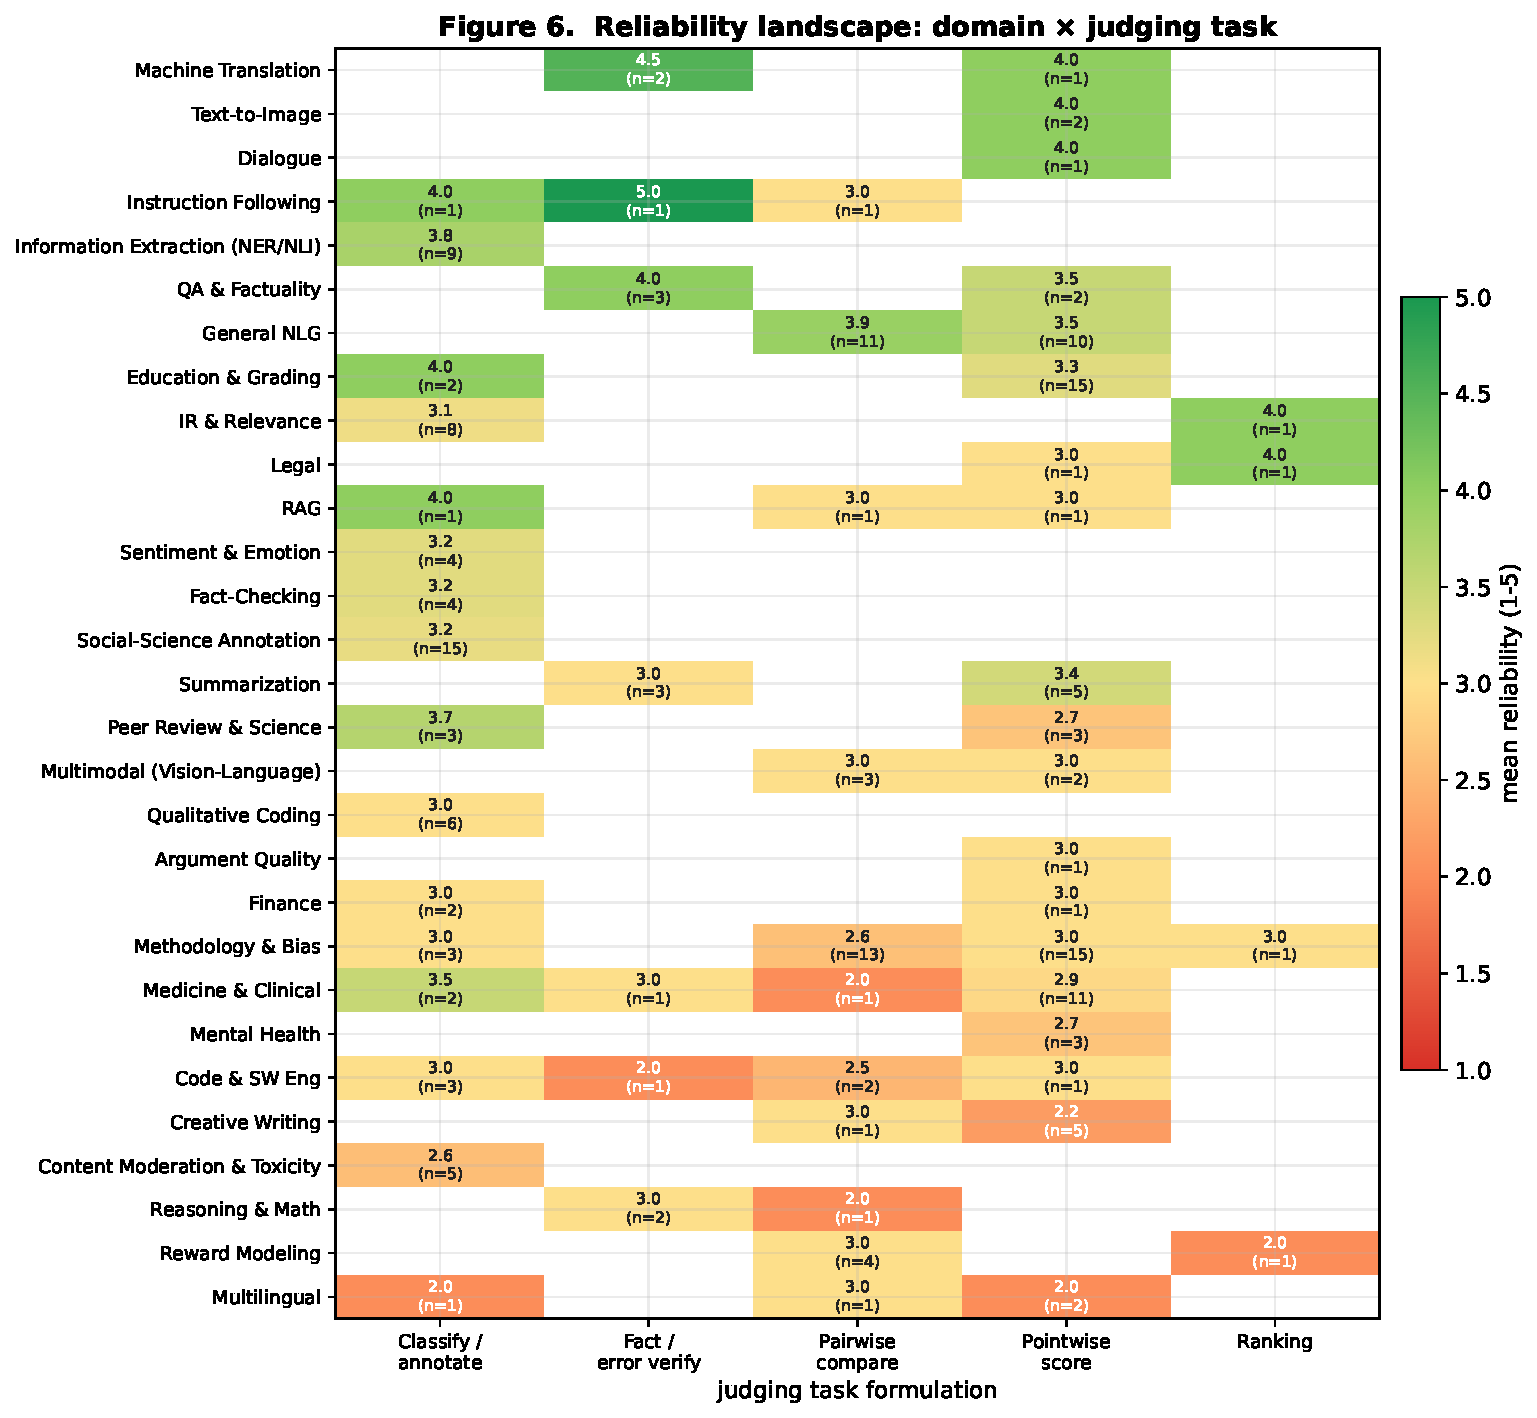
\includegraphics[width=\linewidth]{fig06_reliability_landscape}\caption{}\label{fig:land1}\end{subfigure}
\caption{Study 1a. (a) Mean reliability by domain (green/amber/red). (b) Reliability landscape: domain$\times$judging
task; verification/classification columns are greener than open-ended scoring.}
\end{figure}

\subsection{Failure modes and the decision map}
Recurring biases such as verbosity/length, position, self-preference, style-over-substance, preference leakage,
non-determinism, and the \emph{expertise gap} (judges converge to crowd, not expert, consensus
\citep{bavaresco2024judgebench}) all modulate reliability (Figure~\ref{fig:bias1}). Agreement should be benchmarked
against the human ceiling, which on subjective tasks is itself low (Krippendorff $\alpha<0.35$
\citep{imrit2026iaa}). The Study-1a decision map (Figure~\ref{fig:dec1}) and Table~\ref{tab:decision} translate this into
deployment guidance and motivate both the moving-target test (Study 1b) and the HCC-specific analysis that follows.

\begin{figure}[t]\centering
\begin{subfigure}{0.5\linewidth}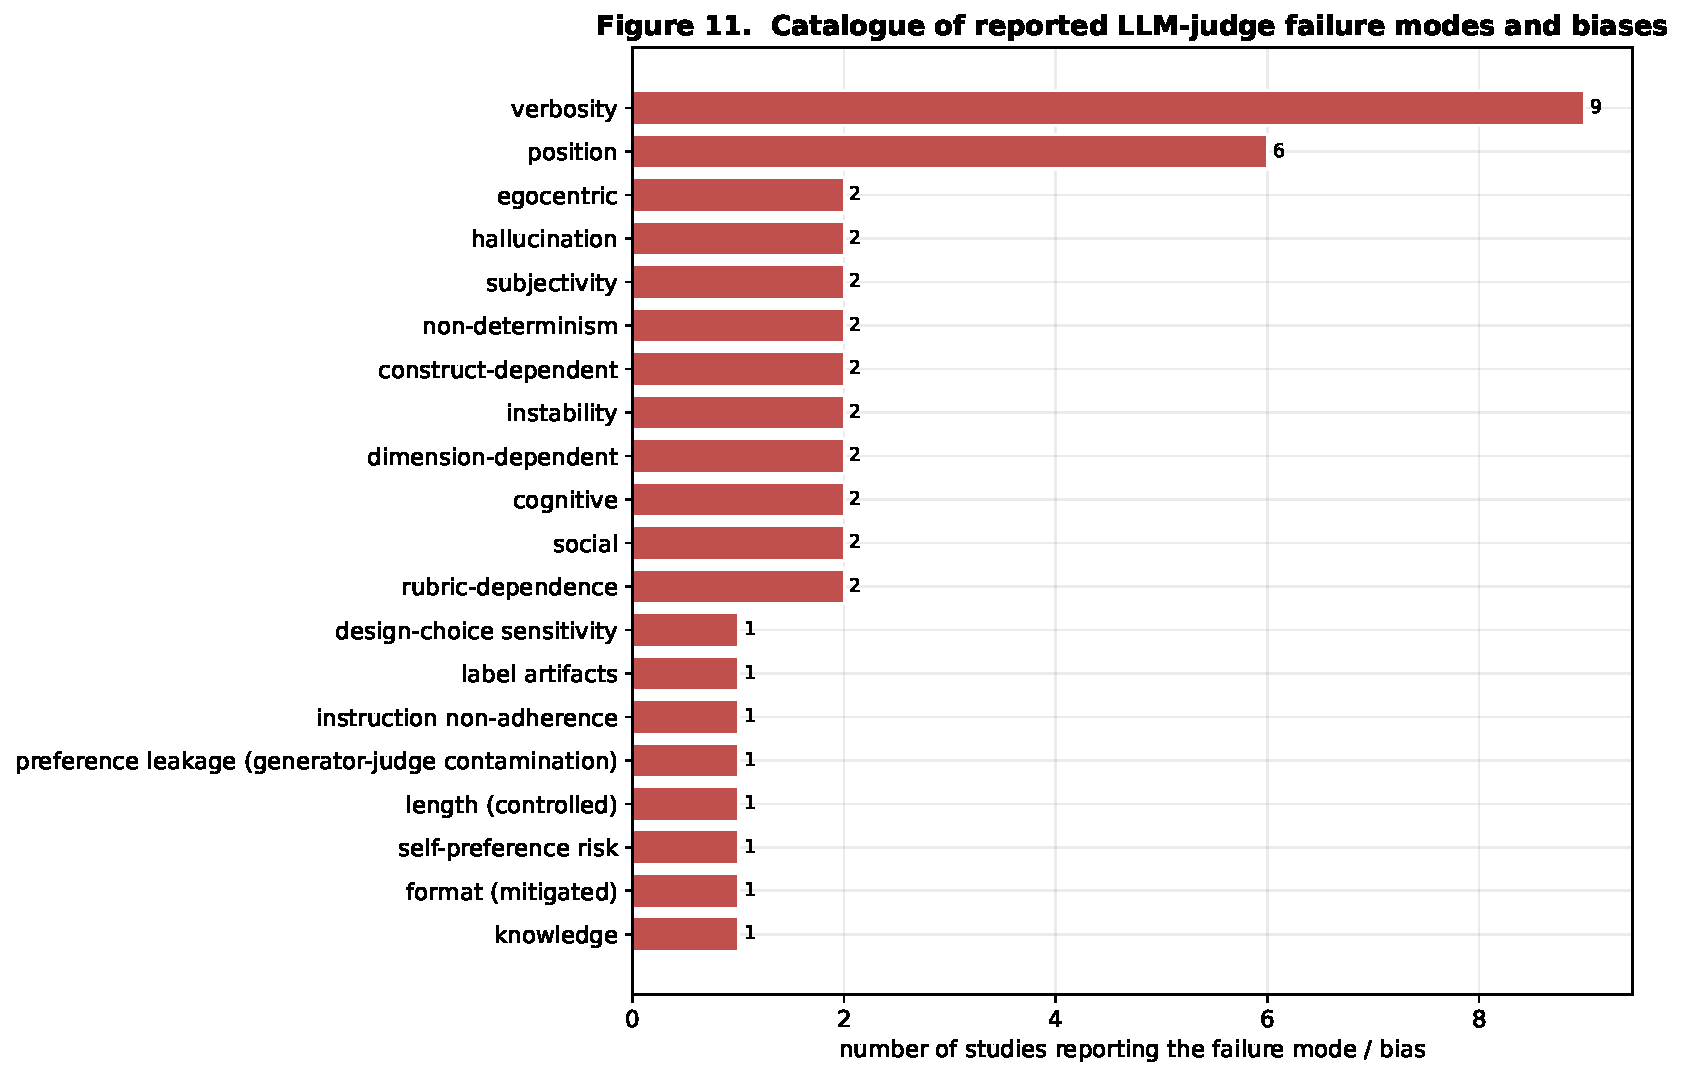
\includegraphics[width=\linewidth]{fig11_bias_frequency}\caption{}\label{fig:bias1}\end{subfigure}\hfill
\begin{subfigure}{0.49\linewidth}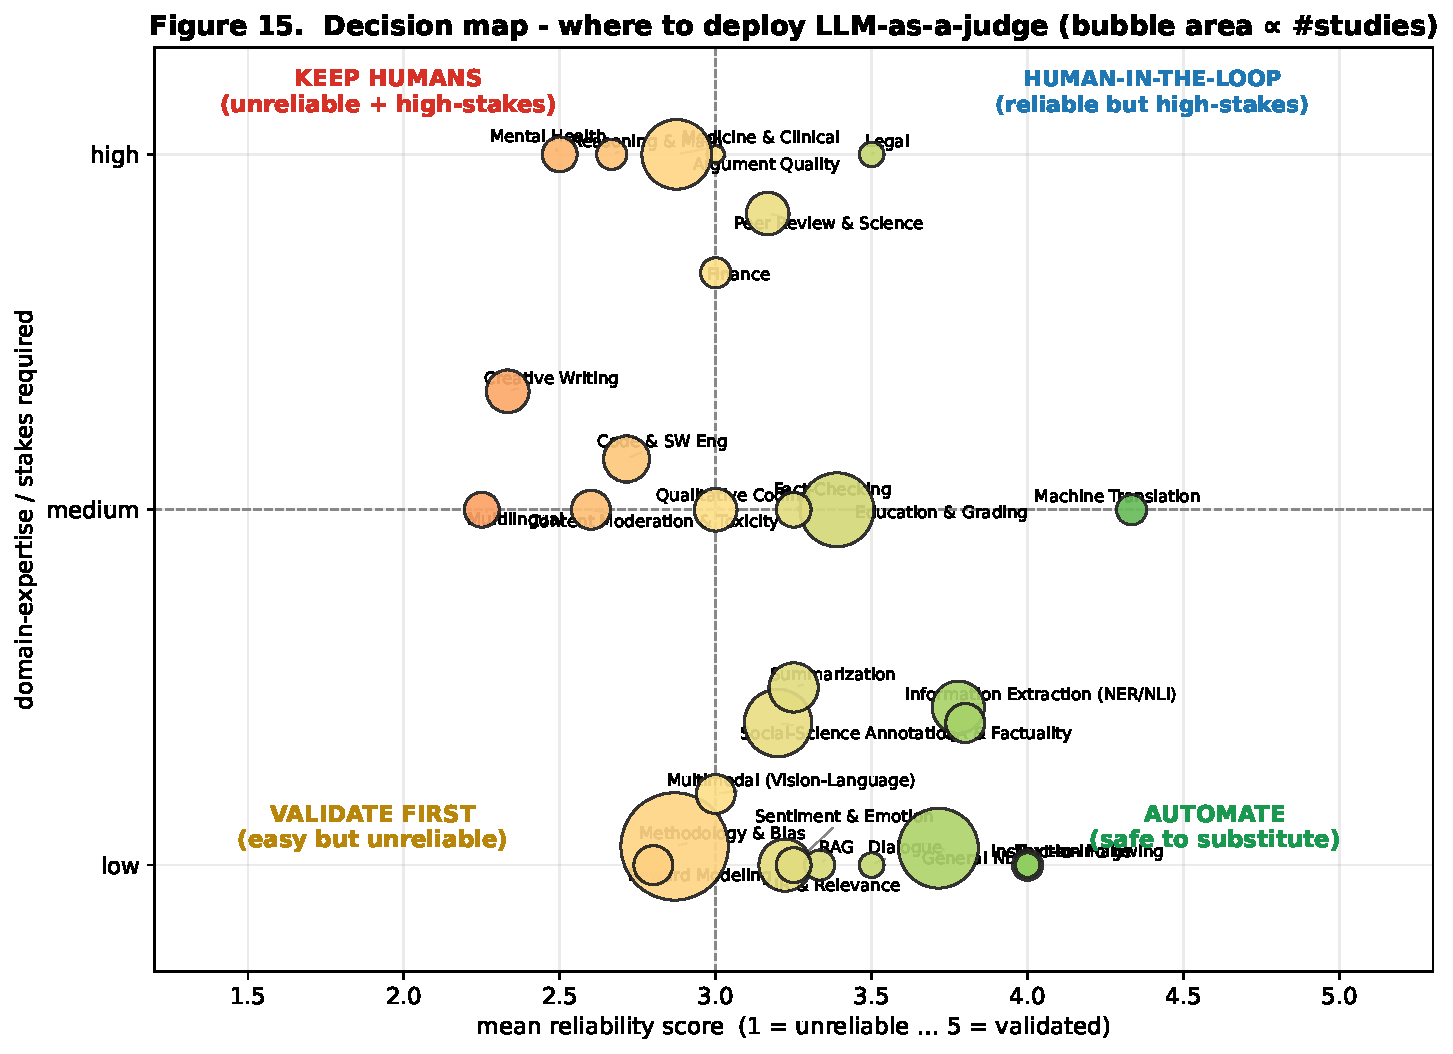
\includegraphics[width=\linewidth]{fig15_decision_map}\caption{}\label{fig:dec1}\end{subfigure}
\caption{Study 1a. (a) Catalogue of reported failure modes/biases. (b) Deployment decision map (reliability$\times$
stakes; bubble area $\propto$ studies).}
\end{figure}

\begin{table}[tbp]\centering\small
\caption{Domain-level decision table. Mean reliability score (1 = unreliable $\dots$ 5 = validated), modal verdict,
and traffic-light signal (\textsc{green} $\ge 3.5$; \textsc{amber} 2.5-3.5; \textsc{red} $<2.5$). Sorted by mean
reliability. Small-$n$ domains should be read together with the family-level aggregates.}
\label{tab:decision}
\begin{tabular}{@{}l r c l c@{}}
\toprule
Domain / task & $n$ & Mean rel. & Modal verdict & Signal \\
\midrule
Machine Translation & 3 & 4.33 & Promising & \cellcolor{g!55}\textsc{green} \\
Text-to-Image & 2 & 4.00 & Promising & \cellcolor{g!55}\textsc{green} \\
Dialogue & 1 & 4.00 & Promising & \cellcolor{g!55}\textsc{green} \\
Instruction Following & 3 & 4.00 & Validated & \cellcolor{g!55}\textsc{green} \\
QA \& Factuality & 5 & 3.80 & Promising & \cellcolor{g!55}\textsc{green} \\
Information Extraction (NER/NLI) & 9 & 3.78 & Promising & \cellcolor{g!55}\textsc{green} \\
General NLG & 21 & 3.71 & Promising & \cellcolor{g!55}\textsc{green} \\
Legal & 2 & 3.50 & Promising & \cellcolor{g!55}\textsc{green} \\
Education \& Grading & 17 & 3.35 & Mixed & \cellcolor{a!60}\textsc{amber} \\
RAG & 3 & 3.33 & Mixed & \cellcolor{a!60}\textsc{amber} \\
Summarization & 8 & 3.25 & Promising & \cellcolor{a!60}\textsc{amber} \\
Fact-Checking & 4 & 3.25 & Promising & \cellcolor{a!60}\textsc{amber} \\
Sentiment \& Emotion & 4 & 3.25 & Mixed & \cellcolor{a!60}\textsc{amber} \\
IR \& Relevance & 9 & 3.22 & Promising & \cellcolor{a!60}\textsc{amber} \\
Social-Science Annotation & 15 & 3.20 & Mixed & \cellcolor{a!60}\textsc{amber} \\
Peer Review \& Science & 6 & 3.17 & Mixed & \cellcolor{a!60}\textsc{amber} \\
Multimodal (Vision-Language) & 5 & 3.00 & Mixed & \cellcolor{a!60}\textsc{amber} \\
Qualitative Coding & 6 & 3.00 & Mixed & \cellcolor{a!60}\textsc{amber} \\
Argument Quality & 1 & 3.00 & Mixed & \cellcolor{a!60}\textsc{amber} \\
Finance & 3 & 3.00 & Mixed & \cellcolor{a!60}\textsc{amber} \\
Medicine \& Clinical & 16 & 2.88 & Mixed & \cellcolor{a!60}\textsc{amber} \\
Methodology \& Bias & 38 & 2.87 & Mixed & \cellcolor{a!60}\textsc{amber} \\
Reward Modeling & 5 & 2.80 & Mixed & \cellcolor{a!60}\textsc{amber} \\
Code \& SW Eng & 7 & 2.71 & Mixed & \cellcolor{a!60}\textsc{amber} \\
Reasoning \& Math & 3 & 2.67 & Mixed & \cellcolor{a!60}\textsc{amber} \\
Content Moderation \& Toxicity & 5 & 2.60 & Mixed & \cellcolor{a!60}\textsc{amber} \\
Mental Health & 4 & 2.50 & Mixed & \cellcolor{a!60}\textsc{amber} \\
Creative Writing & 6 & 2.33 & Mixed & \cellcolor{r!55}\textsc{red} \\
Multilingual & 4 & 2.25 & Caution & \cellcolor{r!55}\textsc{red} \\
\bottomrule
\end{tabular}
\end{table}

% =====================================================================
\section{Study 1b: Is the reliability landscape a moving target?}\label{sec:s1b}
% =====================================================================
A systematic review necessarily captures results \emph{as reported}, and most ``promising''-band evidence in
Study~1a was produced with proprietary judges that are now one or two model generations old (e.g.\ the influential
G-Eval used GPT-4). This raises a question that the review alone cannot answer: when an LLM judge falls short of the
human ceiling in a promising domain, is that a \emph{temporary} limitation that more capable models will erase
(``matter of time''), or a \emph{structural} property of LLM-as-a-judge that better models do not overcome? Study~1b
answers this directly for a flagship case by re-running the evaluation with the most powerful open models available
to us today and comparing against the canonical reported numbers.

\subsection{Method}
We select \textbf{SummEval} \citep{fabbri2021summeval} (summarization quality assessment, a central amber-band task
in Study~1a) because it pairs (i) a widely cited LLM-judge result to beat (G-Eval/GPT-4; \citealp{liu2023geval})
with (ii) public expert human ratings on four aspects (coherence, consistency, fluency, relevance) for
$100\times16=1600$ machine summaries. We replicate the G-Eval summary-level protocol \emph{verbatim} (same aspect
definitions, 1-5 integer ratings, temperature~0) but swap the judge for the \ONEmodels{} most powerful open models
in the available open-model catalogue (\ONEpanel). The comparison metric is the canonical \emph{summary-level Spearman}: for each
source document, correlate the judge's 16 scores with the human means, averaged across documents. The bar to beat is
G-Eval/GPT-4's reported per-aspect correlations (coherence~.582, consistency~.507, fluency~.455, relevance~.547;
average~$\approx$.52). In total Study~1b contributes \ONEnjudg{} fresh judgments.

\subsection{Results}
\begin{table}[t]\centering\small
\caption{Study 1b. Summary-level Spearman $\rho$ of the most powerful open judges on SummEval vs.\ the reported
G-Eval-4/GPT-4 correlations (\ONEnjudg{} judgments). Green cells \emph{surpass} the reported per-aspect number.}
\label{tab:study1b}
\begin{tabular}{@{}l cccc c@{}}
\toprule
Judge & Coher. & Consist. & Fluency & Relev. & Avg $\rho$ \\
\midrule
\textit{Reported (G-Eval-4)} & 0.582 & 0.507 & 0.455 & 0.547 & 0.523 \\
\midrule
\texttt{deepseek-v4-pro} & 0.548 & \cellcolor{g!30}0.688 & 0.392 & 0.540 & \cellcolor{g!30}0.542 \\
\texttt{qwen3.6-35b-a3b} & \cellcolor{g!30}0.606 & \cellcolor{g!30}0.702 & 0.298 & 0.540 & \cellcolor{g!30}0.536 \\
\texttt{glm-5.1} & \cellcolor{g!30}0.650 & \cellcolor{g!30}0.693 & 0.217 & 0.543 & \cellcolor{g!30}0.526 \\
\texttt{gptoss-120b} & \cellcolor{g!30}0.586 & \cellcolor{g!30}0.685 & 0.260 & 0.482 & 0.503 \\
\bottomrule
\end{tabular}
\end{table}
Table~\ref{tab:study1b} reports each open model's summary-level Spearman against the reported G-Eval bar, and
Figure~\ref{fig:s1b} plots them per aspect. \ONEverdictphrase{} \ONEnsurpass{} of the \ONEmodels{} open judges beat
G-Eval's reported \emph{average} correlation, led by \ONEbest{} (avg summary-level $\rho=\ONEbestrho$ vs.\ the
reported ${\approx}\ONEreportedrho$). The aspect pattern is itself the finding. On \textbf{consistency} (the most
\emph{verifiable} judgment, groundable in the source document) \emph{all four} models leap past the reported value
(from $.507$ to $.685$-$.702$), and on \textbf{coherence} three of four do (up to $.650$ vs.\ $.582$);
\textbf{relevance} is on par ($.48$-$.54$ vs.\ $.55$). But on \textbf{fluency} every open model falls well
\emph{short} ($.22$-$.39$ vs.\ a reported $.455$): human fluency ratings of competent machine summaries are
compressed near the top of the scale (low variance), so the summary-level correlation is structurally low
\emph{regardless of how capable the judge is}, a limit that lives in the human reference, not the model, and that
scale does not move.

\begin{figure}[t]\centering
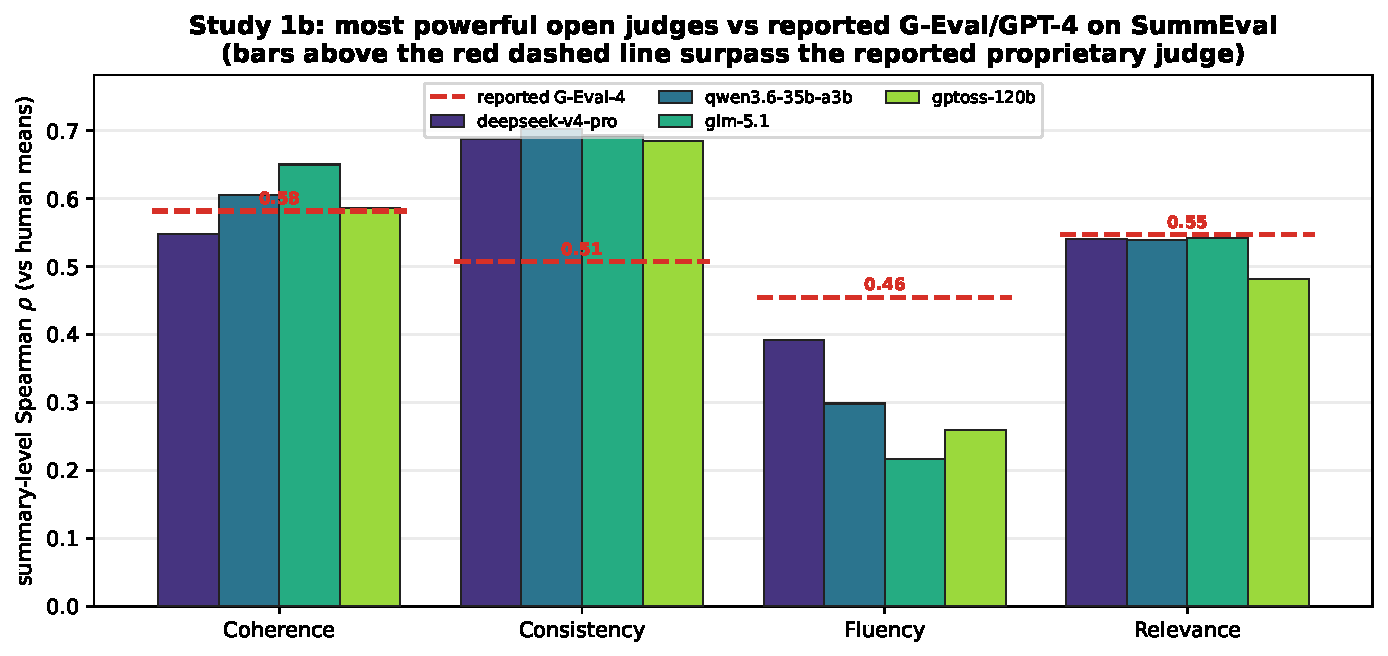
\includegraphics[width=0.97\linewidth]{s1b_fig01_spearman}
\caption{Study 1b. Summary-level Spearman of the most powerful open judges on SummEval, per aspect, against the
reported G-Eval/GPT-4 bar (dashed). Bars above the dashed line indicate an open model that \emph{surpasses} the
reported proprietary-judge correlation.}
\label{fig:s1b}
\end{figure}

\paragraph{Interpretation: time vs.\ structure.} Study~1b shows the reliability landscape is \emph{partly} a moving
target. Where Study~1a's amber rating reflected a capability gap on a verifiable sub-judgment, today's open models
close or exceed it; reliability there is largely a matter of time and access. But where the shortfall reflects a
\emph{compressed or contested human ceiling} (e.g.\ fluency, and, as Study~3 will show, subjective social annotation),
even the most powerful models do not break through, because the limit lives in the human reference, not the model.
This distinction, temporal capability gap vs.\ structural ceiling, is the lens we carry into HCC.

\paragraph{Takeaway for HCC.} Study~1a says LLM judges are safe where the task is objective and verifiable, and
Study~1b shows that frontier open models are now strong enough to match proprietary judges on exactly those
verifiable tasks. But HCC's signature methods (qualitative interpretation, participant study, design
judgment) are precisely the \emph{subjective, expert, interpretive} tasks Study~1a flags as risky and Study~1b
predicts scale will \emph{not} fix. Study~2 tests whether that prediction holds in the HCC literature itself.

% =====================================================================
\section{Study 2: LLM substitution in HCC, HCI, and qualitative methods}
% =====================================================================
\subsection{Motivation and research questions}
Study 1's map is domain-general; HCC needs a method-specific account. Human-centered research is built on methods
that historically \emph{require} human input: qualitative coding, thematic and content analysis, interviews and
open-ended survey analysis, crowdsourced annotation, participant studies, persona development, usability/heuristic
evaluation, and design critique. Study 2 asks: \textbf{(RQ2.1)} which of these methods have been attempted with
LLMs, and how reliably do LLM outputs agree with human input? \textbf{(RQ2.2)} How does the field position the
LLM, to \emph{augment}, \emph{replace}, or \emph{simulate} the human? \textbf{(RQ2.3)} What epistemic stance
(enabling, tension, critical) does the literature take, and what does that imply for HCC practice?

\subsection{Method}
Following the shared protocol, we ran a Study-2-specific identification arm: 25 HCC/HCI/qualitative concept-block
queries against OpenAlex (\SToa{} unique works), triangulated with the web arm and with the venue-scoped sweep of
Study 1 (CHI, CSCW, UIST, IUI, TOCHI). After topicality screening and eligibility assessment we included
\STN{} studies (Figure~\ref{fig:s2prisma}). We extracted, per study: the HCC \textbf{method}; the LLM \textbf{role}
(replace / augment / simulate); reported agreement and the human baseline; the reliability \textbf{verdict};
the \textbf{epistemic stance} (enabling / tension / critical); and the \textbf{community} (HCI, CSCW,
qualitative-methods, computational social science, NLP, health). The full corpus is \sttwotabref.

\begin{figure}[t]\centering
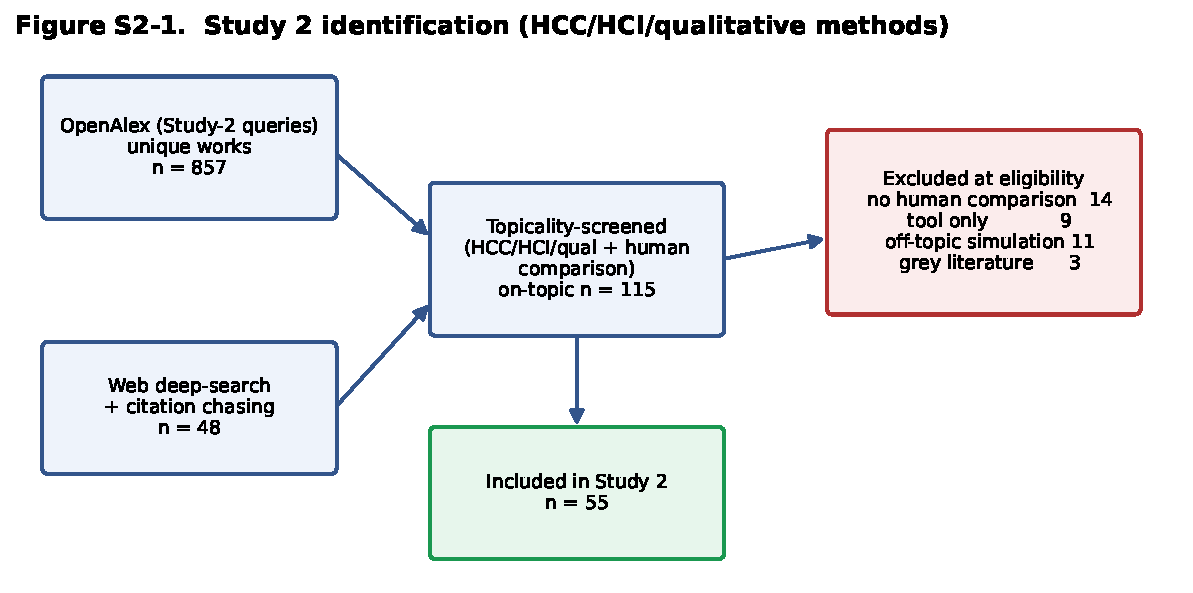
\includegraphics[width=0.96\linewidth]{s2_fig01_prisma}
\caption{Study 2 identification flow (HCC/HCI/qualitative methods).}
\label{fig:s2prisma}
\end{figure}

\subsection{RQ2.1: Which methods, and how reliable?}
LLMs have been compared against human input across \STmethods{} distinct HCC methods
(Figure~\ref{fig:s2methods}), most heavily in \emph{thematic analysis}, \emph{synthetic participants}, and
\emph{crowdsourced annotation}. Reliability is strongly method-dependent (Figure~\ref{fig:s2relmethod};
Table~\ref{tab:s2methods}). The \emph{same objectivity/interpretation axis} from Study 1 governs HCC:
\textbf{objective crowd-annotation} is the most reliable method to substitute: ChatGPT matches or beats crowd
workers and even trained coders on stance, topic, and frame labeling \citep{gilardi2023chatgpt,tornberg2023political};
\textbf{deductive/inductive coding and content/thematic analysis} are reliable \emph{as augmentation}, with
human-equivalent agreement on structured codebooks (GPT-4 exceeding substantial $\kappa$ on 8/9 hermeneutic tasks
\citep{dunivin2024scalablecot}; Gemini $\kappa=0.907$ in multi-LLM thematic analysis \citep{jain2025multillmthematic};
79.7\% agreement in health thematic summarization \citep{castellanos2025thematicsumm}) but only moderate agreement
in open interpretive settings ($\kappa\approx0.40$-$0.46$ \citep{li2024gpt4humanqual,qualcoding2025jla}); and
\textbf{participant/persona simulation and usability evaluation} are the least reliable.

\begin{figure}[t]\centering
\begin{subfigure}{0.52\linewidth}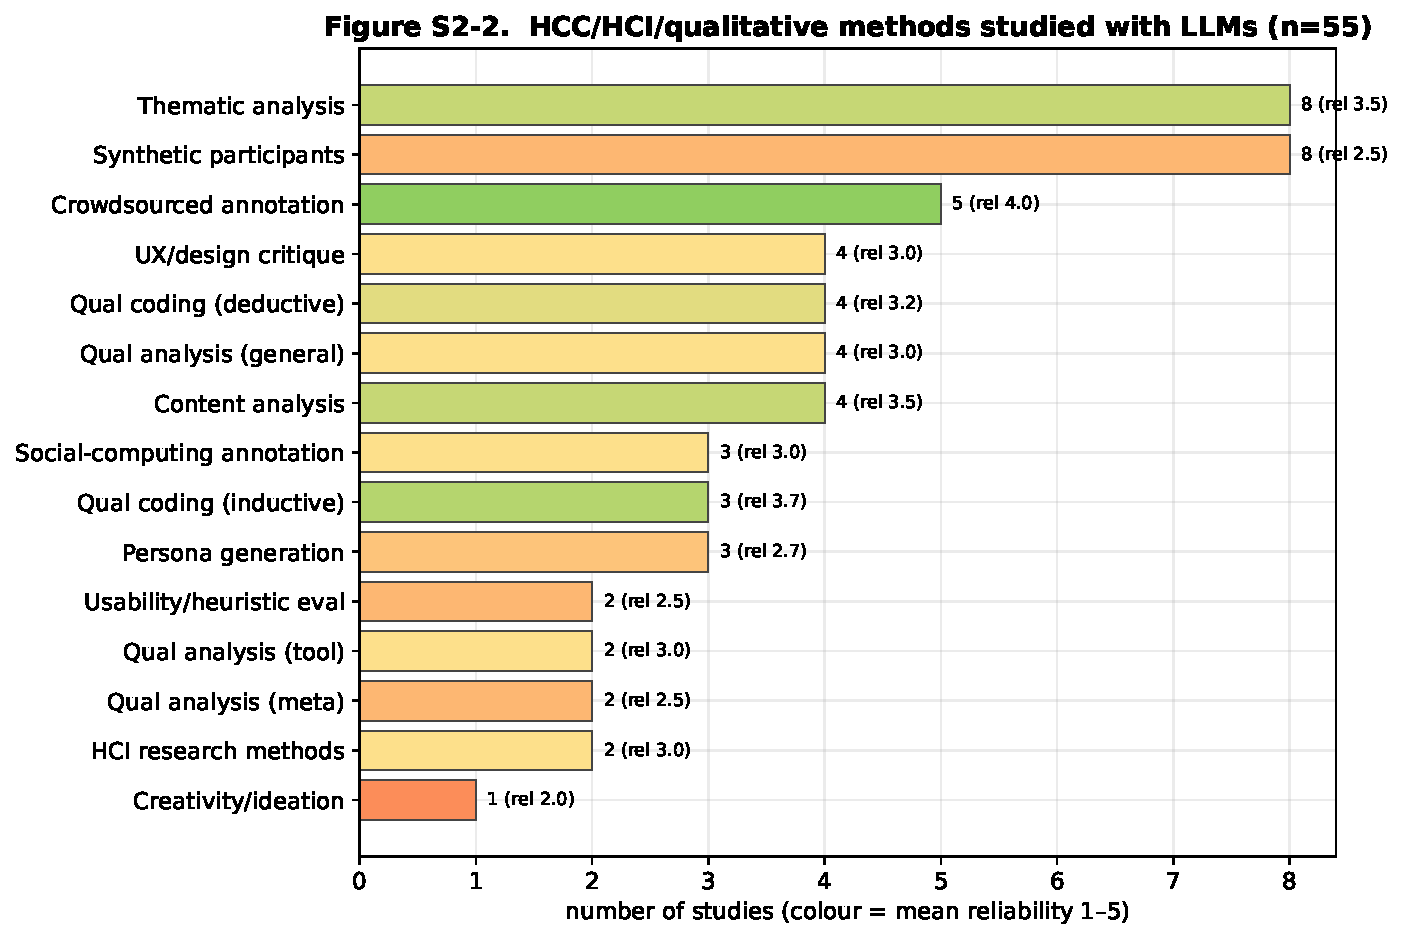
\includegraphics[width=\linewidth]{s2_fig02_methods}\caption{}\label{fig:s2methods}\end{subfigure}\hfill
\begin{subfigure}{0.46\linewidth}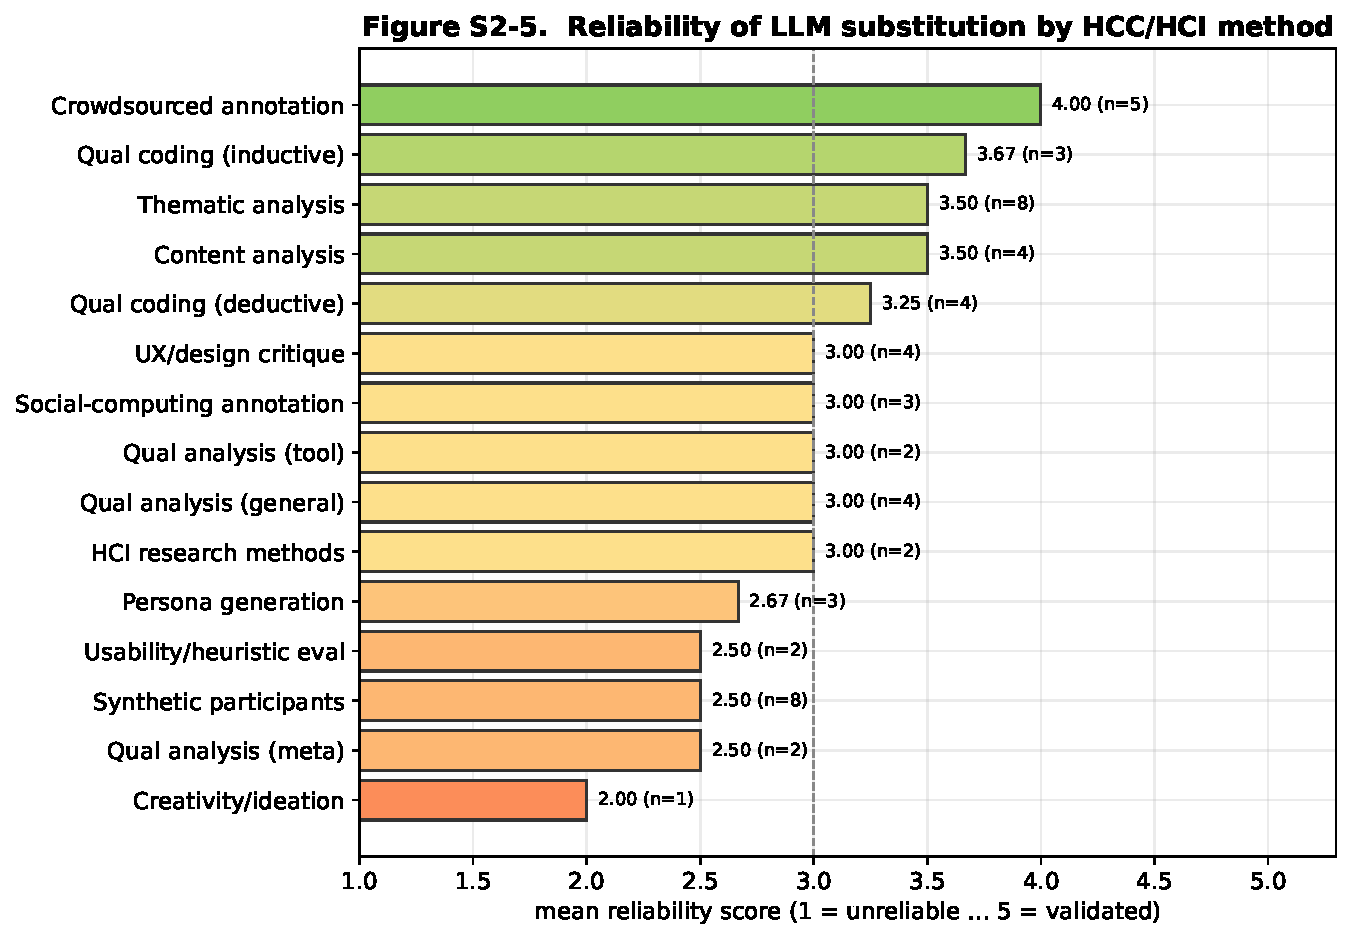
\includegraphics[width=\linewidth]{s2_fig05_reliability_by_method}\caption{}\label{fig:s2relmethod}\end{subfigure}
\caption{Study 2. (a) HCC/HCI/qualitative methods studied with LLMs (colour = mean reliability). (b) Mean reliability
of LLM substitution by method.}
\end{figure}

\begin{table}[t]\centering\small
\caption{Study 2 method-level decision table: study count, modal LLM role, mean reliability, and traffic-light
signal (\textsc{green} $\ge3.5$; \textsc{amber} 2.5-3.5; \textsc{red} $<2.5$).}
\label{tab:s2methods}
\begin{tabular}{@{}l r l c c@{}}
\toprule
Method & $n$ & Modal role & Mean rel. & Signal \\
\midrule
Crowdsourced annotation & 5 & replace & 4.00 & \cellcolor{g!55}\textsc{green} \\
Qual coding (inductive) & 3 & augment & 3.67 & \cellcolor{g!55}\textsc{green} \\
Content analysis & 4 & augment & 3.50 & \cellcolor{g!55}\textsc{green} \\
Thematic analysis & 8 & augment & 3.50 & \cellcolor{g!55}\textsc{green} \\
Qual coding (deductive) & 4 & augment & 3.25 & \cellcolor{a!60}\textsc{amber} \\
HCI research methods & 2 & augment & 3.00 & \cellcolor{a!60}\textsc{amber} \\
Qual analysis (general) & 4 & augment & 3.00 & \cellcolor{a!60}\textsc{amber} \\
Qual analysis (tool) & 2 & augment & 3.00 & \cellcolor{a!60}\textsc{amber} \\
Social-computing annotation & 3 & replace & 3.00 & \cellcolor{a!60}\textsc{amber} \\
UX/design critique & 4 & augment & 3.00 & \cellcolor{a!60}\textsc{amber} \\
Persona generation & 3 & augment & 2.67 & \cellcolor{a!60}\textsc{amber} \\
Qual analysis (meta) & 2 & augment & 2.50 & \cellcolor{a!60}\textsc{amber} \\
Synthetic participants & 8 & simulate & 2.50 & \cellcolor{a!60}\textsc{amber} \\
Usability/heuristic eval & 2 & replace & 2.50 & \cellcolor{a!60}\textsc{amber} \\
Creativity/ideation & 1 & augment & 2.00 & \cellcolor{r!55}\textsc{red} \\
\bottomrule
\end{tabular}
\end{table}

\subsection{RQ2.2: Augment, replace, or simulate?}
HCC overwhelmingly positions LLMs to \emph{augment} humans, not replace them: \STaugment{} of \STN{} studies frame
the LLM as a collaborator/assistant, versus \STreplace{} as a replacement and \STsimulate{} as a human simulator
(Figure~\ref{fig:s2rolestance}a). This is not merely rhetorical caution; it tracks reliability
(Figure~\ref{fig:s2verdictrole}): augmentation studies skew reliable, whereas \emph{replacement} is validated only
for objective annotation and \emph{simulation} of participants is the least reliable role
(mean reliability augment \STrelaugment{} vs.\ replace \STrelreplace{} vs.\ simulate \STrelsim{}). The replacement
mean is buoyed by objective crowd-annotation; remove it and replacement of \emph{interpretive} human input is
firmly amber/red. The canonical HCC workflow that emerges is human-in-the-loop: LLM proposes, human vets and retains
interpretive authority \citep{gao2024collabcoder,meng2024chalet,dai2023llminloop}.

\begin{figure}[t]\centering
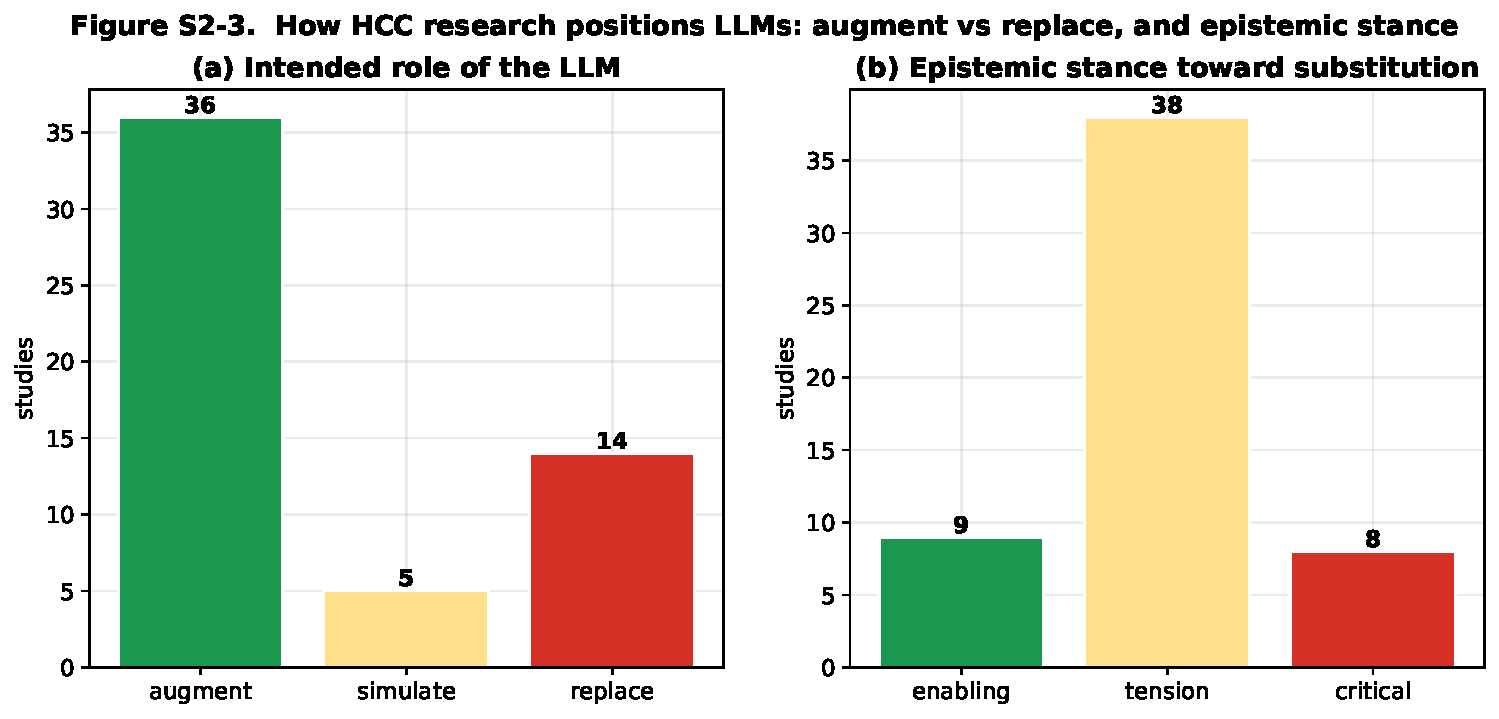
\includegraphics[width=0.95\linewidth]{s2_fig03_role_stance}
\caption{Study 2. (a) Intended LLM role across the HCC corpus; augmentation dominates. (b) Epistemic stance toward
substitution; \emph{tension} dominates.}
\label{fig:s2rolestance}
\end{figure}

\begin{figure}[t]\centering
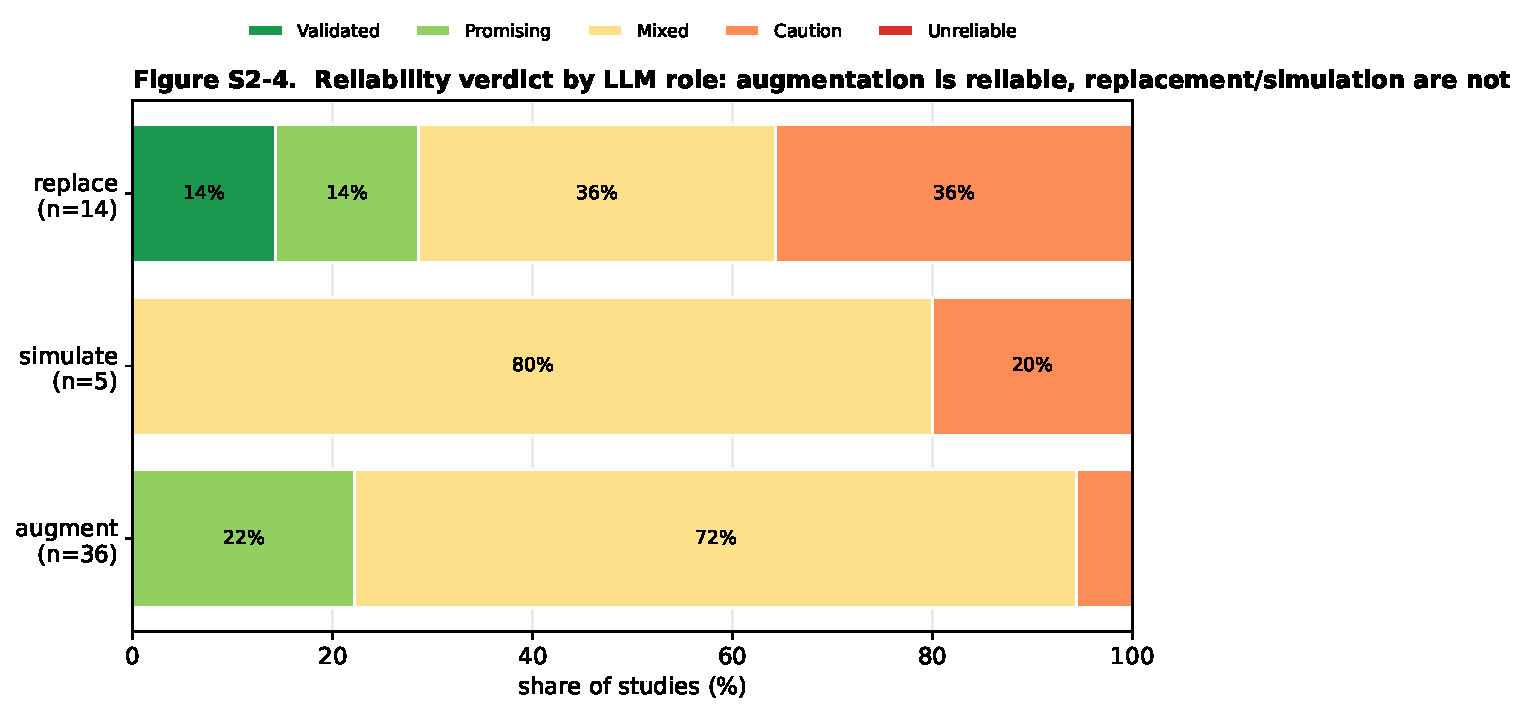
\includegraphics[width=0.8\linewidth]{s2_fig04_verdict_by_role}
\caption{Study 2. Reliability verdict by LLM role. Augmentation is reliable; replacement is reliable only for
objective annotation; participant/usability \emph{simulation} is the least reliable.}
\label{fig:s2verdictrole}
\end{figure}

\subsection{RQ2.3: Epistemic stance and the limits of substitution}
The dominant stance is \emph{tension} (\STtension/\STN), with \STcritical{} explicitly \emph{critical} and only
\STenabling{} unreservedly \emph{enabling} (Figure~\ref{fig:s2rolestance}b). Three threads recur.
\textbf{(i) Interpretation and reflexivity.} Qualitative scholars warn that LLMs perform surface-level extraction
well but cannot supply the situated, reflexive interpretation that gives qualitative findings their validity, and
that ``conditional trust'' in tool output risks hollowing out analytic rigor \citep{schroeder2025usestensions,
ngo2026chatqda,davison2024ethics,nguyentrung2025chatgptta}.
\textbf{(ii) Participants and identity.} Replacing human participants with LLMs \emph{flattens and misportrays}
demographic groups, positionality cannot be simulated \citep{wang2024flatten}, and LLM ``subgroups'' are often
caricatures \citep{cheng2023compost}; synthetic survey data distort variances and correlations
\citep{bisbee2023perils}, and an LLM is worth only a bounded number of real respondents \citep{huang2025surveyworth}.
HCI critiques accordingly recast synthetic users as ``objects of inquiry,'' not stand-ins \citep{salminen2025syntheticcritical,
haxvig2025personabias}.
\textbf{(iii) Expert design judgment.} GPT-4o overlaps only 21\% with expert-found usability issues and hallucinates
false positives \citep{guerino2025gpt4ousability}, and LLM UI critique trails expert designers
\citep{duan2024uicrit}, though synthetic heuristic evaluation can exceed \emph{novice} evaluators on issue recall
\citep{zhong2025synthheuristic}. Figure~\ref{fig:s2comm} shows coverage skews to HCI and computational social
science, with the augment-replace reliability gap visible across communities.

\begin{figure}[t]\centering
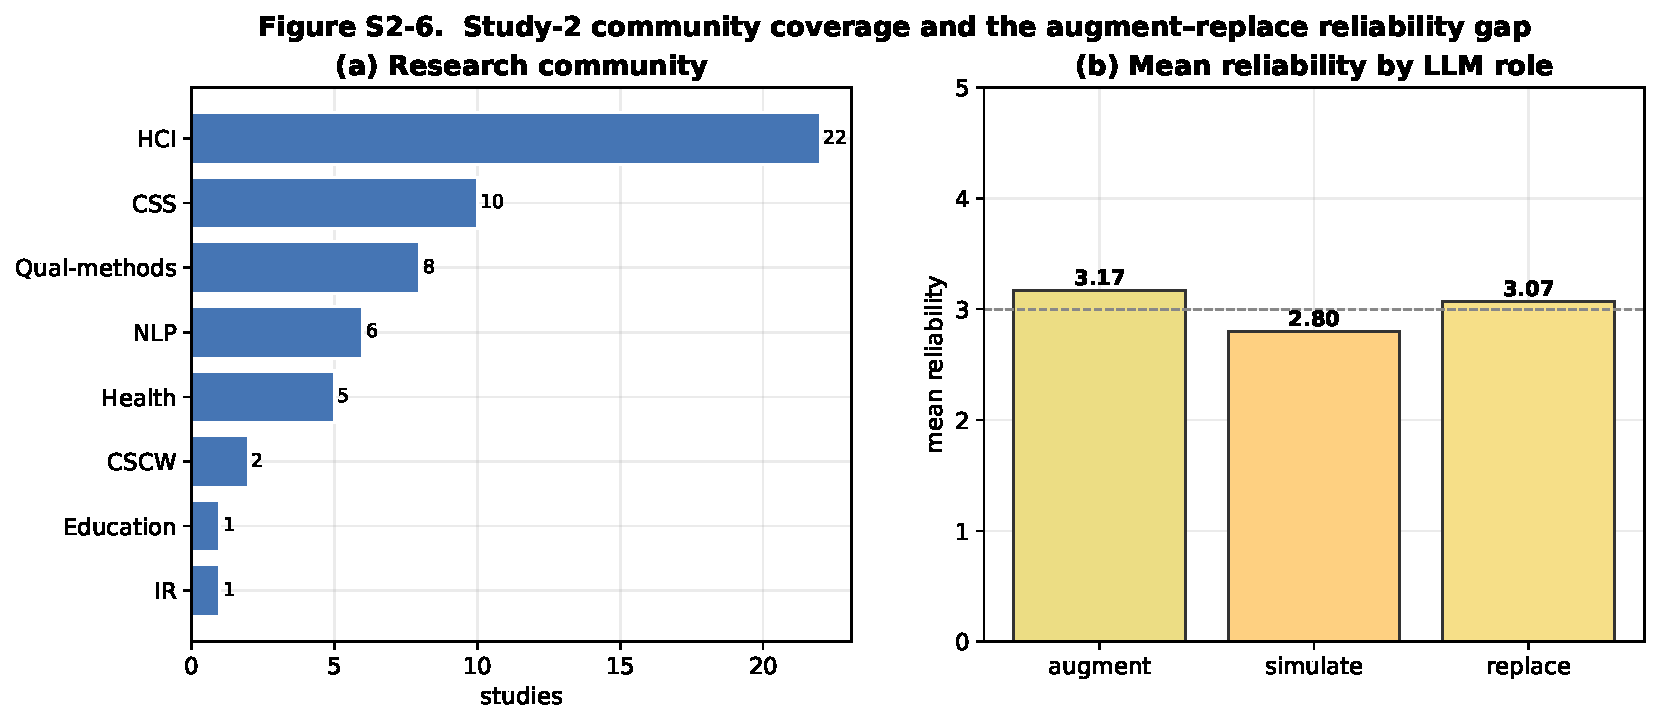
\includegraphics[width=0.95\linewidth]{s2_fig06_community_role}
\caption{Study 2. (a) Coverage by research community. (b) Mean reliability by LLM role, augmentation $>$
replacement $>$ simulation.}
\label{fig:s2comm}
\end{figure}

\subsection{Study 2 synthesis}
For HCC research, the evidence supports a clear, conditional posture.
\textbf{Validated to substitute:} objective crowd/data annotation (stance, topic, relevance, frames) where a human
ceiling is modest and verifiable.
\textbf{Reliable only as augmentation (human-in-the-loop):} deductive/inductive qualitative coding and thematic/
content analysis: LLMs accelerate breadth and first-pass coding, but humans must own interpretation, theme
development, and reflexive accounting.
\textbf{Unsafe to substitute:} simulating human participants, generating personas as stand-ins for real users, and
replacing expert usability/design judgment: these flatten identity, fabricate issues, and forfeit the situated
knowledge that defines human-centered inquiry. This posture both confirms Study 1's objective/subjective prediction
\emph{within} HCC and exposes concrete gaps (\S\ref{sec:study3}) where HCC datasets with human labels have never
been formally tested with an LLM judge.

% =====================================================================
\section{Study 3: An empirical LLM-as-a-judge evaluation on HCC datasets with human ground truth}
\label{sec:study3}
% =====================================================================
Studies 1-2 expose a recurring gap: many human-centered datasets ship with human labels yet have never had a
\emph{formal} LLM-as-a-judge evaluation, meaning a panel of models, bias controls, agreement benchmarked against the
human ceiling, and a contamination check. Study 3 closes this gap empirically with a released, reproducible harness.

\subsection{Method}
We evaluate a panel of \STHRmodels{} open models served via \textbf{\PROVIDER{}} (OpenAI-compatible),
spanning five families and 9B-754B parameters (\texttt{glm-5.1}~754B, \texttt{gptoss-120b}, \texttt{deepseek-v4},
\texttt{gemma-4-31b}, \texttt{qwen3.6-27b}, \texttt{qwen3.5-9b}), run in parallel at each model's documented
concurrency. Each model judges every item as a \emph{virtual annotator} under the same instructions the humans
received. We benchmark against the \emph{human-human ceiling} (random-annotator-vs-majority accuracy and pairwise
agreement, computed from the per-item annotator counts), report accuracy, Cohen's $\kappa$, and macro-F1 against the
majority gold, compute a count-based \textbf{alt-test} winning rate \citep{calderon2025alttest}, aggregate the panel
into a majority \textbf{jury} \citep{verga2024poll}, and run a verbatim quote-completion \textbf{contamination
probe}. Sample size is power-justified at $n{=}500$ items/dataset (95\% CI half-width $\le\!\pm4.4\%$; $>$80\% power
for a 0.10 gap vs the ceiling). The run comprised \textbf{\STHRn{} judgments} across \STHRdatasets{} datasets with
\emph{zero} API errors and a 100\% answer-parse rate; only item-level labels and aggregates are released (no raw
text), and the two sensitive sets are used under their public licenses.

\subsection{Results}
Figures~\ref{fig:s3acc}-\ref{fig:s3heat} and Table~\ref{tab:study3} yield one organizing finding:
\textbf{the human-agreement ceiling governs LLM reliability.} Where humans agree little (NLI; ceiling 0.64-0.75) the
panel \emph{matches or exceeds} them: on ChaosNLI-SNLI 5/6 models are \textbf{Validated} (jury 0.858 $>$ ceiling
0.752), and ChaosNLI-MNLI is \textbf{Promising}. Where humans agree strongly on a subjective social construct, the panel falls
short: GoEmotions 4-way sentiment (ceiling 0.78) is uniformly \textbf{Mixed} (best 0.61); HateXplain 3-way hate
(ceiling 0.835) is \textbf{Mixed} at best and \textbf{Unreliable} for the small model; binary offensiveness (SBIC,
ceiling 0.905) is the strongest social-computing case (\textbf{Promising}; \texttt{glm-5.1} 0.856) yet still below
the ceiling. The sixth dataset is a deliberate \emph{clean condition}: MultiPICo irony detection
\citep{casola2024multipico}, a 2024 perspectivist corpus recent enough to be unlikely in pretraining. Its human
ceiling is itself low (0.82, just above the 76\% majority baseline); the panel \emph{matches} it
(\textbf{Promising}; best 0.82, jury 0.83) but largely by defaulting to the majority class (macro-F1 ${\approx}0.45$),
and \texttt{qwen3.5-9b} collapses (0.40, \textbf{Unreliable}). Four further effects: (i) \textbf{granularity}: binary offensiveness (Promising) clearly beats 3-way
hate (Mixed); (ii) \textbf{scale}: \texttt{qwen3.5-9b} is weakest on \emph{every} dataset (Caution/Unreliable),
while 27B-754B cluster together (bigger is not always better: 31B \texttt{gemma} ties the 754B \texttt{glm});
(iii) the \textbf{alt-test} (winning rate $\ge$0.5) is passed only on the \emph{low-ceiling} tasks, NLI and the
binary irony set (5/6 models on both ChaosNLI-SNLI and MultiPICo); on every \emph{high-consensus} task, including the
Promising binary offensiveness (SBIC, 0/6), no model earns the statistical right to replace a human annotator;
(iv) \textbf{juries}
raise accuracy but do not lift any subjective task above its human ceiling. The \textbf{contamination probe}
(Table~\ref{tab:study3}, last column) shows the strongest judges have non-trivial verbatim recall across sets
(gemma MEDIUM throughout), caveating the NLI ``Validated'' result; crucially the recent low-contamination MultiPICo
(LOW for the small-recall \texttt{qwen3.5-9b}) is still matched only at its low human ceiling, so the
social-computing shortfall tracks the human ceiling, not memorization.

\begin{figure}[t]\centering
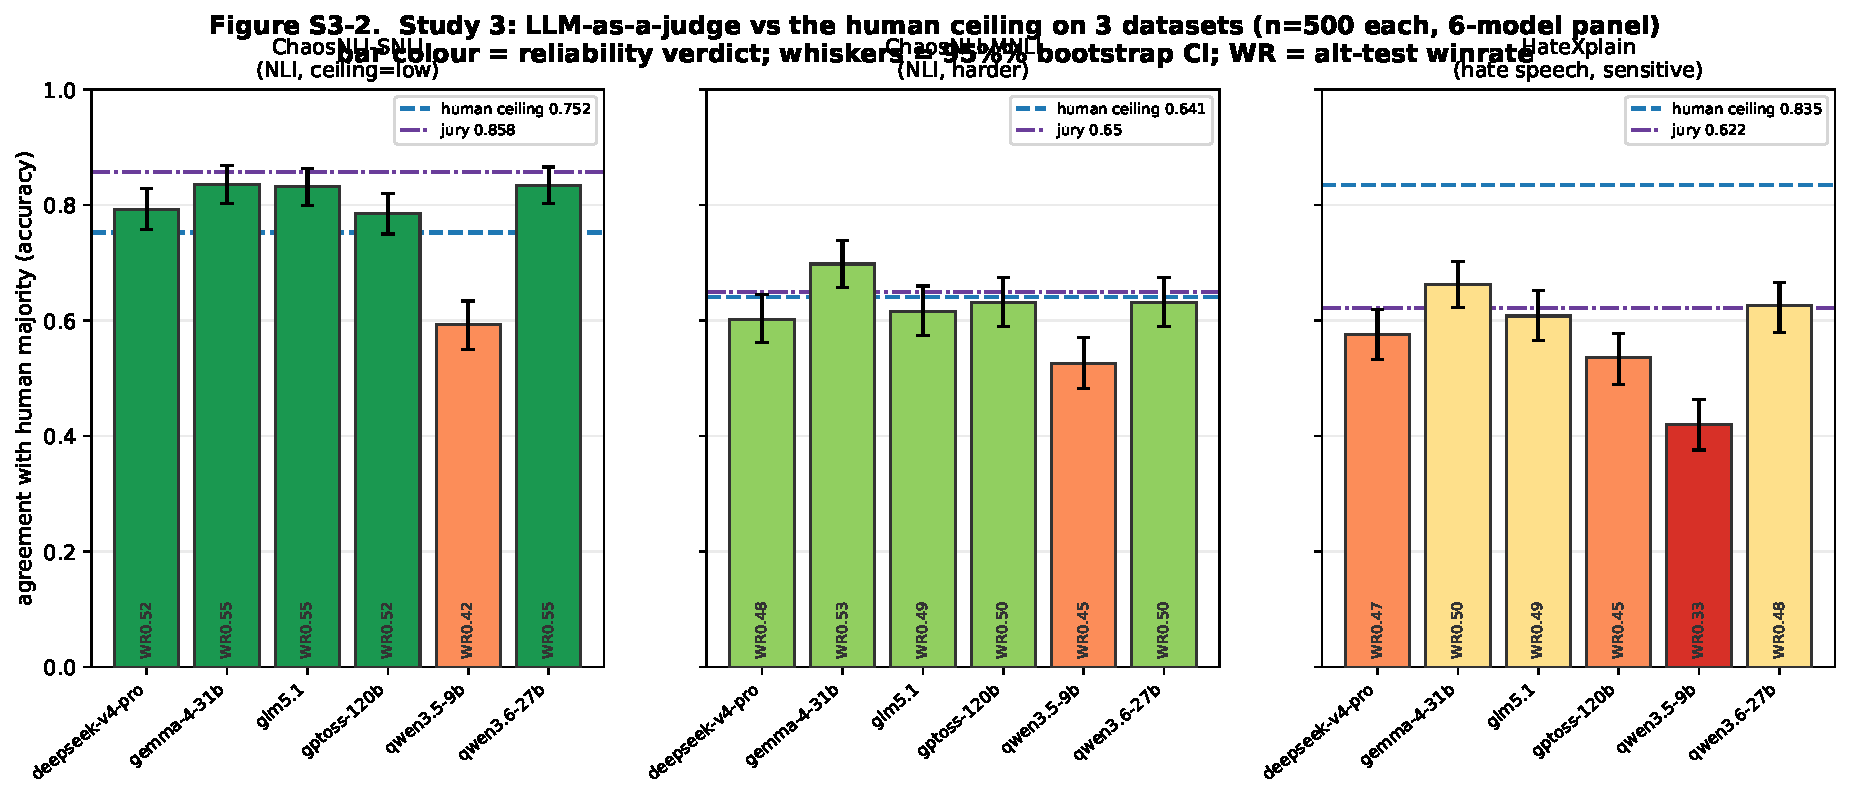
\includegraphics[width=\linewidth]{s3_fig02_full_accuracy}
\caption{Study 3. Per-dataset accuracy vs the human ceiling (blue dashed) for the 6-model panel (n=500 each;
whiskers = 95\% bootstrap CI; bar colour = verdict; WR = alt-test winning rate). Datasets ordered by construct
subjectivity. LLMs clear LOW ceilings (NLI) but fall short of HIGH ceilings on subjective social-computing tasks.}
\label{fig:s3acc}
\end{figure}

\begin{figure}[t]\centering
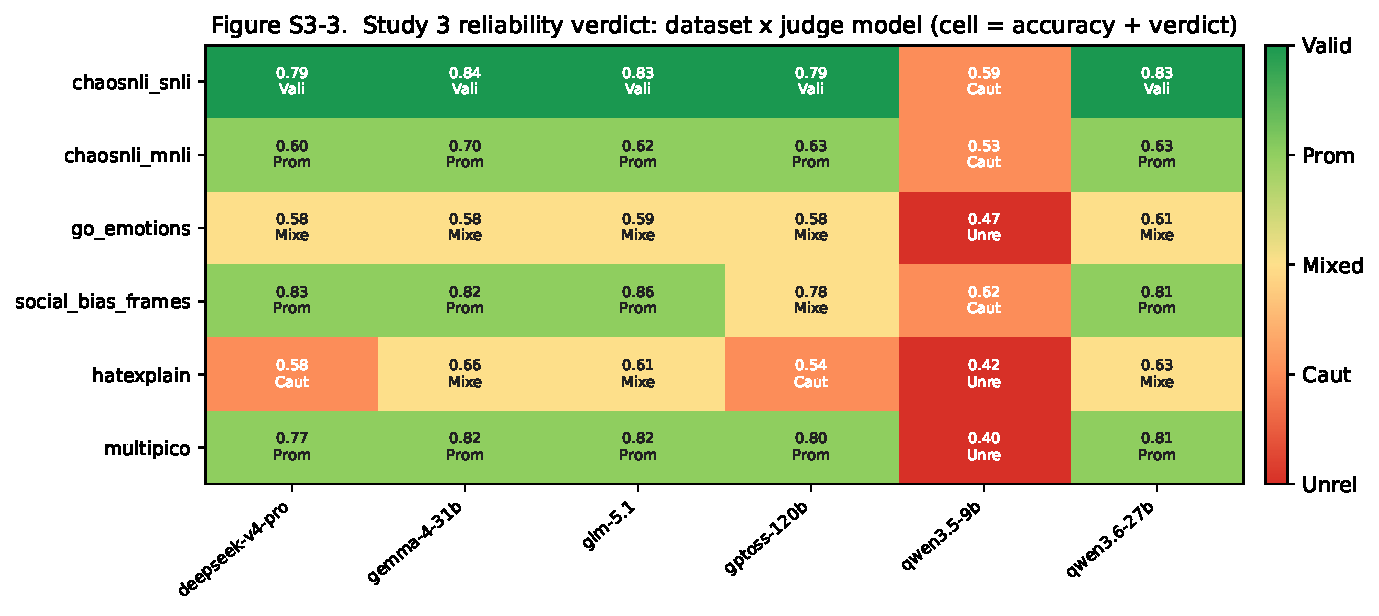
\includegraphics[width=0.92\linewidth]{s3_fig03_full_verdict}
\caption{Study 3. Dataset$\times$judge-model reliability verdict (cell = accuracy + verdict). The scale effect
(\texttt{qwen3.5-9b} column) and the construct-subjectivity gradient (rows) are both visible.}
\label{fig:s3heat}
\end{figure}

\begin{table}[t]\centering\small
\caption{Study 3 results across \STHRdatasets{} datasets $\times$ \STHRmodels{} models (\STHRn{} judgments).
Human ceiling = random-annotator-vs-majority accuracy; alt-test pass = winning rate $\ge0.5$; contamination tier
from the verbatim-recall probe.}
\label{tab:study3}
\begin{tabular}{@{}l l c c c c l c@{}}
\toprule
Dataset & Construct & Human & Best model & macro-F1 & Jury & Modal verdict & Contam. \\
 & & ceiling & (acc) & (best) & (acc) & & tier \\
\midrule
ChaosNLI-SNLI & NLI & 0.75 & 0.84 (gemma-4-31b) & 0.79 & 0.86 & \cellcolor{g!55}Validated & MEDIUM \\
ChaosNLI-MNLI & NLI & 0.64 & 0.70 (gemma-4-31b) & 0.70 & 0.65 & \cellcolor{g!25}Promising & MEDIUM \\
GoEmotions & emotion (4-way) & 0.78 & 0.61 (qwen3.6-27b) & 0.54 & 0.61 & \cellcolor{a!60}Mixed & MEDIUM \\
SBIC & offensive (binary) & 0.91 & 0.86 (glm-5.1) & 0.85 & 0.84 & \cellcolor{g!25}Promising & MEDIUM \\
HateXplain & hate (3-way) & 0.83 & 0.66 (gemma-4-31b) & 0.64 & 0.62 & \cellcolor{a!60}Mixed & MEDIUM \\
MultiPICo (clean) & irony (binary) & 0.82 & 0.82 (gemma-4-31b) & 0.70 & 0.83 & \cellcolor{g!25}Promising & MEDIUM \\
\bottomrule
\end{tabular}
\end{table}

\subsection{What governs reliability? A mixed-effects analysis}
To test the ``ceiling governs'' claim inferentially rather than descriptively, we model every individual judgment
($N{=}\STHRn$; outcome $=\mathbf{1}[\text{judge}=\text{majority gold}]$) with a logistic specification whose fixed
effects are task \emph{subjectivity} ($1\!-\!$human-ceiling accuracy, at the dataset level) and model \emph{scale}
($\log_{10}$ parameters), reported both as a Bayesian mixed-effects logistic GLMM with random intercepts for dataset
and item, and, for clean inference, as a logistic GLM with item-cluster-robust standard errors
(Figure~\ref{fig:s3stats}). Three results stand out. (i) \textbf{Subjectivity dominates:} each unit of
$1\!-\!$ceiling multiplies the odds of agreeing with humans by $\mathrm{OR}=\SMEsubjOR$ ($p=\SMEsubjP$). (ii)
\textbf{Scale helps, but modestly:} larger models do better ($\mathrm{OR}=\SMEsizeOR$ per $\log_{10}$ params,
$z=\SMEsizeZ$), an effect far smaller than subjectivity's, consistent with Study~1b's ``partly a moving target.''
(iii) \textbf{Variance lives in the items:} the GLMM random-intercept standard deviation is far larger across
\emph{items} ($\mathrm{SD}=\SMEvcitem$) than across datasets ($\mathrm{SD}=\SMEvcdataset$), i.e.\ \emph{which item}
is being judged, its latent human (dis)agreement, explains judge correctness better than which model judges or
even which dataset it comes from. Finally, a Benjamini-Hochberg analysis across all \SMEfdrtests{}
judge$\times$dataset cells finds \SMEfdrsig{} significant at $q<.05$: \textbf{\SMEfdrbelow{} sit significantly
\emph{below} the human ceiling} and only \SMEfdrabove{} significantly above (the objective-NLI cases). Scaling the
judge shifts cells modestly rightward; it does not move a high-ceiling subjective task across the line.

\begin{figure}[t]\centering
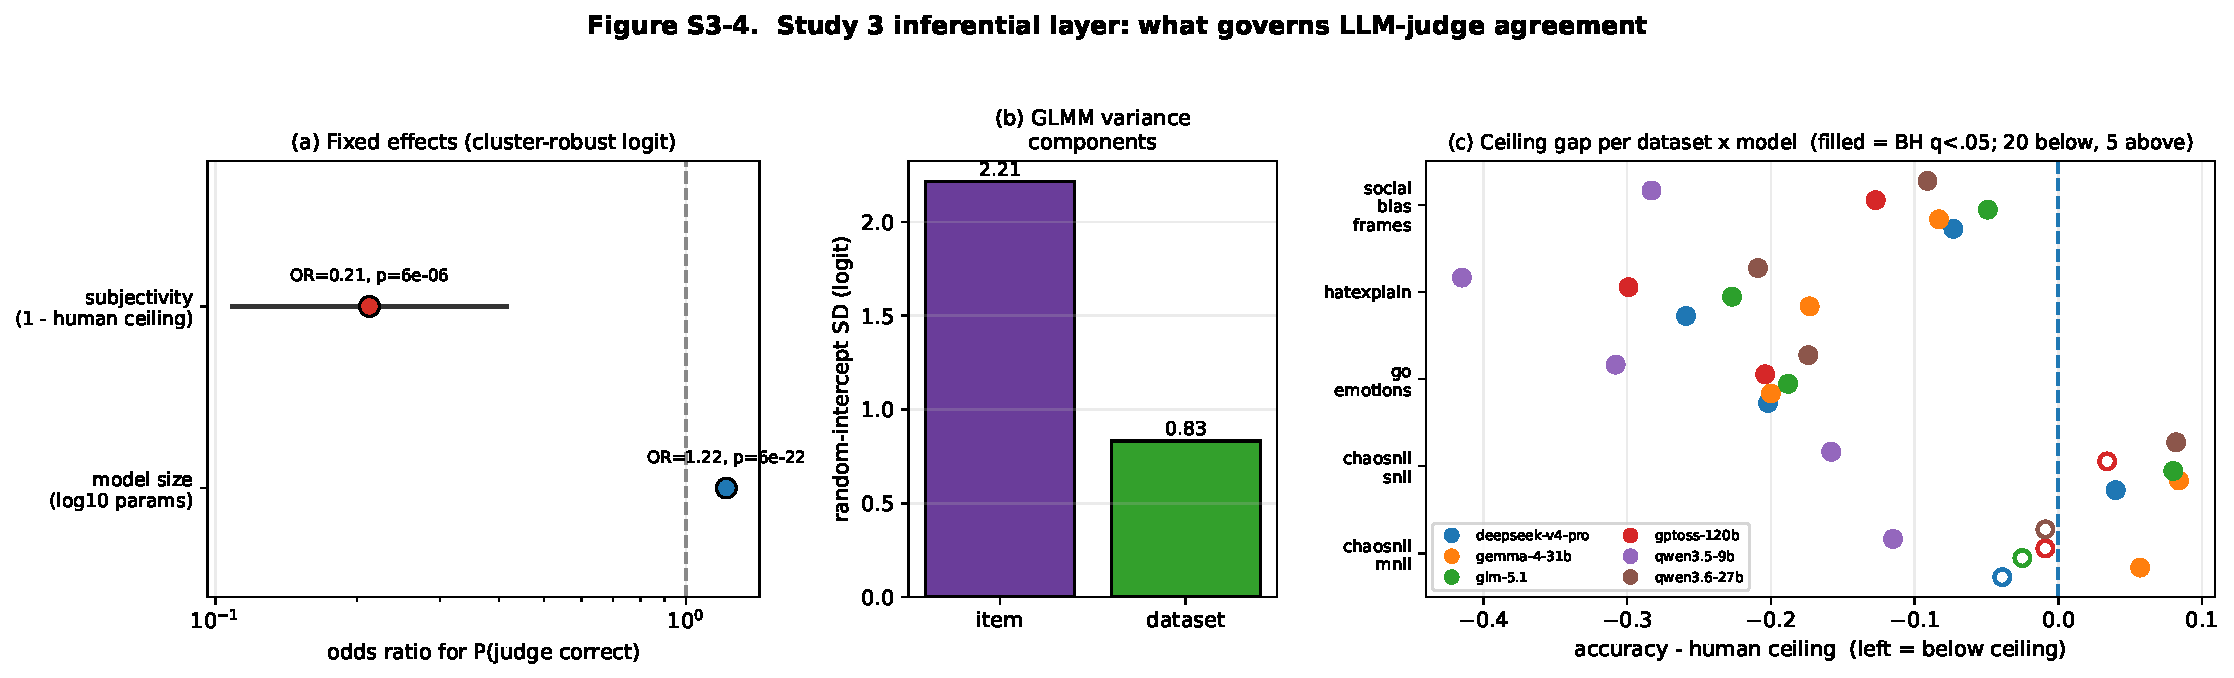
\includegraphics[width=\linewidth]{s3_fig04_stats}
\caption{Study 3 inferential layer. (a) Fixed-effect odds ratios (item-cluster-robust logit): subjectivity is a
strong negative predictor of judge correctness, scale a weak positive one. (b) GLMM variance components: item-level
variance dominates. (c) Ceiling gap per judge$\times$dataset (filled = BH $q<.05$); most cells sit below the human
ceiling.}
\label{fig:s3stats}
\end{figure}

\subsection{Integration with the decision framework}
Mapped onto the five-level rubric, Study 3 drops fresh, dataset-level points into the Study-1/2 landscape and
\emph{quantitatively confirms} the augment-not-replace conclusion for human-centered annotation: LLM judges are a
validated substitute for objective/low-ceiling labeling and a strong assistant for coarse (binary) moderation, but
fall short of, and fail the replacement test for, subjective, fine-grained, or high-consensus human-centered
constructs, a pattern the mixed-effects model shows is driven by item-level human (dis)agreement rather than by
model scale. The recent MultiPICo clean condition rules out contamination as the explanation: a 2024 set the
low-recall judge has not memorized is still matched only at its (low) human ceiling. \emph{Limitation:} the panel is
limited to open models from a single provider, and qualitative-coding corpora with public multi-coder labels (still
scarce) are the immediate next addition.

% =====================================================================
\section{Discussion}
% =====================================================================

\subsection{From four research questions to one principle}
Our studies were designed as a narrowing sequence, and their research questions answer one another.
\textbf{Study 1a} asked \emph{where}, across domains, an LLM-as-a-judge agrees with humans; its goal was to give HCC
a map and a vocabulary, and it found that reliability tracks three properties (objectivity, tractable verification,
and a low human-agreement floor). \textbf{Study 1b} asked whether that map is a \emph{moving target}; its goal was
to separate temporal from structural limits, and it found that today's most powerful open models already match or
exceed proprietary judges on the \emph{verifiable} part of a promising task (consistency on SummEval) but not on the
part whose human ceiling is compressed (fluency), so capability closes some gaps and cannot close others.
\textbf{Study 2} asked, of the methods HCC actually uses, which have been attempted with LLMs and how reliably
(RQ2.1), how the field positions the model as augment/replace/simulate (RQ2.2), and with what epistemic stance
(RQ2.3); its goal was the HCC-specific account, and it found an augment-not-replace consensus whose reliability
follows the same objective/subjective axis as Study 1a, under a dominant stance of \emph{tension}. \textbf{Study 3}
asked whether that prediction holds when measured directly on HCC datasets with human labels, and \emph{what governs}
the outcome; its goal was to fill the empirical gaps and identify the mechanism, and it found that the
human-agreement ceiling governs reliability, that item-level disagreement (not model scale, and not contamination)
is the dominant source of variance, and that even the strongest panel fails the alt-test wherever humans agree
strongly.

These answers converge on a single principle that we offer as the paper's organizing contribution:
\begin{quote}\itshape
An LLM-as-a-judge can be reliable only to the degree that the human task has a high, verifiable agreement ceiling;
it cannot exceed an agreement level that human annotators themselves do not reach, and scaling the model does not
raise that ceiling.
\end{quote}
This reframes the field's animating question. ``Can a machine judge like a human?'' is under-specified; the
answerable question is \emph{whether there is a stable, shared human answer for the judge to approximate}. Where
there is (objective labeling, verifiable sub-judgments), frontier models already clear the bar; where there is not
(interpretation, identity, contested constructs), no amount of capability manufactures a ground truth that the human
community does not itself possess.

\subsection{Connections to HCI and measurement scholarship}
Our results give empirical weight to three long-running conversations in HCI and adjacent fields.
\textbf{(1) The myth of a single ground truth.} CSCW and HCI have argued that inter-rater reliability is a negotiated
practice, not a natural fact \citep{mcdonald2019reliability}, and NLP has reframed annotator disagreement as
signal rather than noise \citep{aroyo2015truth,plank2022humanlabel}. Study 3 operationalizes this: when we benchmark
judges against the human-human ceiling rather than a manufactured ``gold,'' the ostensibly poor performance on
emotion, hate, and irony is revealed as a property of the \emph{construct} (low or contested human consensus), not a
fixable model deficiency. A judge that reports high accuracy against a forced majority is, on these tasks, reporting
agreement with a coin the humans themselves are still flipping.
\textbf{(2) Interpretation is not labeling.} Reflexive thematic analysis treats coding as situated interpretation,
not classification \citep{braun2006thematic}, and qualitative HCI scholars warn that ``conditional trust'' in LLM
output hollows out analytic rigor \citep{schroeder2025usestensions,davison2024ethics}. Study 2's augment-not-replace
consensus and Study 3's subjective-task shortfall are two views of the same boundary: LLMs accelerate the
\emph{mechanical} surface of qualitative work while the interpretive core remains human.
\textbf{(3) Participants are not simulable.} The ``silicon sample'' program \citep{argyle2023outofone} meets a
growing critique that simulated participants flatten identity and distort variance
\citep{wang2024flatten,cheng2023compost,bisbee2023perils,salminen2025syntheticcritical}; our MultiPICo result, where
models default to the majority reading and erase the minority perspective that perspectivist corpora were built to
preserve, is a concrete instance of that flattening at the level of a single subjective label.

\subsection{A critical assessment: what these practices do to the field}
We read the rush to LLM-as-a-judge in HCC as carrying five structural risks that the community should name.
\textbf{Illusory validation.} Because agreement on older public benchmarks can reflect memorization rather than
competence, ``validated'' verdicts are not trustworthy without a contamination check; our probe shows non-trivial
verbatim recall even of recent data, and a field that omits this step risks certifying judges that merely remember.
\textbf{Methodological monoculture and deskilling.} Cheap labeling invites the substitution of LLM judgment for the
human annotation and reflexive interpretation that train the next generation of HCC researchers; combined with the
documented convergence of judges toward crowd rather than expert consensus \citep{bavaresco2024judgebench}, this
risks a slow regression of the field's interpretive capacity toward the mean of its own training data.
\textbf{Epistemic injustice and flattening.} Where models default to majority readings of subjective content, the
perspectives of minority annotators (often the populations HCC seeks to center) are systematically discounted, a
representational harm that a single accuracy number conceals.
\textbf{False closure on contested constructs.} Reporting one accuracy against a majority gold imposes consensus
where the data shows disagreement; our irony case (0.82 accuracy but macro-F1 near 0.45) shows how a high headline
number can mask the fact that the model has learned the base rate, not the construct.
\textbf{Incentive capture.} The very convenience of LLM evaluation pressures authors, reviewers, and venues to treat
it as a default, embedding its biases into the published record. Against these we weigh genuine benefits, scale,
triage, breadth, reproducibility, first-pass coding, and disagreement surfacing, and conclude that LLM judges should
be governed as \emph{instruments requiring calibration and disclosure}, not adopted as oracles.

\subsection{Implications for designing experiments that use LLM-as-a-judge}
The same evidence yields concrete, reusable guidance. We recommend that any study using an LLM-as-a-judge:
\begin{enumerate}[leftmargin=1.5em,itemsep=2pt]
\item \textbf{Anchor to the human-human ceiling, not a single gold.} Report the ceiling (e.g.\ random-annotator-vs-
majority and pairwise agreement) and the judge-vs-ceiling gap; ``near-human'' is meaningless without it.
\item \textbf{Gate replacement claims on a replacement test.} Report the alt-test \citep{calderon2025alttest} (or an
equivalent leave-one-annotator-out test) before asserting that an LLM can stand in for a human annotator.
\item \textbf{Probe contamination} for any public or pre-cutoff dataset, and discount validation under high recall;
state model training-cutoff relative to dataset release.
\item \textbf{Match the metric to the construct.} On imbalanced or minority-sensitive tasks report macro-F1 and
per-class scores, and prefer disagreement-aware evaluation against the full label distribution (soft labels) over
forced-majority accuracy.
\item \textbf{Control known biases and pin the setup.} Counterbalance position, control length, check
self-preference, and fix model identifier, version, decoding (temperature, seed) so the judge is reproducible.
\item \textbf{Power the comparison.} Pre-specify the effect size of interest, report confidence intervals, and size
$n$ accordingly; our analysis shows variance lives at the item level, so also \emph{stratify by item difficulty} and
report where the judge fails rather than only its mean.
\item \textbf{Use juries for aggregate decisions, but not as a ceiling-breaker.} Panels improve stability yet do not
lift a subjective task above its human ceiling.
\item \textbf{Pre-register and release.} Register the construct, the human baseline, and the decision threshold; and
release item-level labels and aggregates so others can re-anchor and re-code.
\end{enumerate}
Adopted together, these move LLM-as-a-judge from an ad hoc convenience to a measured instrument with a known
operating range, which is the precondition for the field to use it without quietly degrading its own standards of
evidence.

\subsection{A decision framework for HCC}
Mapping the principle onto practice yields three deployment regimes:
\begin{itemize}[leftmargin=1.4em,itemsep=2pt]
\item \textbf{Automate (with light audit):} objective annotation/labeling of user-generated content such as
stance, topic, relevance, frames, and simple sentiment \citep{gilardi2023chatgpt,tornberg2023political}, where the
ceiling is high and verifiable.
\item \textbf{Augment, human-in-the-loop:} qualitative coding and thematic/content analysis: use the LLM for
first-pass coding, breadth, and disagreement surfacing, but keep human interpretive authority, calibrate on a
labeled subset, and report reliability against human coders \citep{gao2024collabcoder,meng2024chalet,
pangakis2023validation}.
\item \textbf{Keep humans (do not substitute):} simulating participants or replacing them with personas, and
replacing expert usability/design judgment: these flatten identity, fabricate evidence, and abandon situated
knowledge \citep{wang2024flatten,guerino2025gpt4ousability,salminen2025syntheticcritical}.
\end{itemize}

% =====================================================================
\section{Limitations}
% =====================================================================
Both reviews used a single-reviewer, LLM-assisted pipeline (logs released) rather than dual human reviewers; metrics
are heterogeneous and synthesized within families rather than pooled; several methods/domains rest on small $n$
(flagged via family/role aggregates); database recall depends on indexing and query phrasing (mitigated, not
removed, by three-source triangulation); and findings reflect models available through mid-2026. The empirical
studies are bounded too: Study 1b uses one flagship promising-domain benchmark (SummEval), and Study 3's panel is
limited to open models from a single provider and to \STHRdatasets{} datasets (one of which, MultiPICo, is included
as a recent low-contamination clean condition), with qualitative-coding corpora still in progress. The verdict
rubric, though explicit and released, embeds judgement; we therefore release both corpora for re-coding. Full
protocol, rubric anchors, dataset cards, verbatim judging prompts, and metric definitions are given in
Appendices~\ref{app:protocol} to~\ref{app:s3detail}.

% =====================================================================
\section{Ethics and reproducibility}
% =====================================================================
\textbf{Ethics.} Studies 1a and 2 analyze published research, not human subjects. Study 3 reuses public datasets
under their licenses; two of them (HateXplain, SBIC) contain hateful or offensive text, which we process only to
measure moderation reliability and never reproduce. To avoid redistributing potentially harmful or
personally-identifiable content, we release only item-level labels and aggregate statistics, never the raw texts. We
report a contamination probe precisely so that ``validated'' verdicts are not silently inflated by pretraining
exposure. The work is dual-use only in the benign sense that better-calibrated LLM judges reduce, rather than
increase, the risk of unaccountable automated moderation; our central finding (that LLM judges should not replace
humans on subjective, high-consensus social annotation) is itself a guard against premature deployment.
\textbf{Reproducibility.} Every number in this paper regenerates from released code: the OpenAlex, Semantic Scholar,
and web search logs; the two coded corpora; the figure and table generators; the Study-1b SummEval harness and the
Study-3 judging/scoring/contamination/mixed-effects harness, all keyed to documented model identifiers served through
\PROVIDER{} at temperature~$0$ with idempotent, resumable checkpoints. The auto-generated statistics macros
mean the manuscript cannot drift from the data. Repository: \REPO{}.

% =====================================================================
\section{Conclusion}
% =====================================================================
LLMs are already remaking how Human-Centered Computing research is done. Our four studies show that this is neither
to be embraced nor refused wholesale. Across \Nstudies{} cross-domain studies and \STN{} HCC-specific studies, the
evidence converges on a conditional verdict: an LLM-as-a-judge is a \emph{validated substitute} for objective
annotation, a \emph{valuable human-in-the-loop assistant} for qualitative coding and analysis, and an
\emph{unsafe replacement} for human participants, personas, and expert design judgment. Study 1b shows that the most
powerful open models now match or exceed proprietary judges on the verifiable parts of ``promising'' tasks, and
Study 3 turns the remaining ``mixed'' verdicts into dataset-level evidence using open, locally-servable models and
the field's own reliability standards. The right question for HCC is never ``can a machine judge?'' but ``\emph{can this machine
replace a second human, on this method, at this granularity, under these controls?}'', and this paper makes that
question answerable, method by method.

\section*{Reproducibility}
Two coded corpora (Study 1: \Nstudies{} studies; Study 2: \STN{} studies), three search logs, PRISMA counts, all
figure/table-generation code, the auto-generated statistics, and the Study-3 evaluation harness are released.
Everything regenerates via \texttt{make all}.


\bibliographystyle{plainnat}
\bibliography{references}

\appendix
\section{Study 1 corpus}\label{app:s1}
{\footnotesize\footnotesize
\begin{longtable}{@{}l l l l l c l@{}}
\caption{Full extracted-studies corpus (217 included studies). Agreement is the headline coefficient/proportion where reported.}\label{tab:full}\\
\toprule
Key & Study & Domain & Task & Metric & Agree & Verdict \\
\midrule
\endfirsthead
\toprule Key & Study & Domain & Task & Metric & Agree & Verdict \\ \midrule \endhead
\texttt{mirzakhmedova2024argument} & Mirzakhmedova et al. (2024) & Argument Quality & pointwise & pct\_agreement & - & Mixed \\
\texttt{tong2024codejudge} & Tong et al. (2024) & Code \& SW Eng & classify & accuracy & - & Promising \\
\texttt{watson2024aicodereview} & Watson et al. (2024) & Code \& SW Eng & classify & pct\_agreement & - & Mixed \\
\texttt{codespec2025} & Jin et al. (2025) & Code \& SW Eng & verify & accuracy & - & Caution \\
\texttt{wang2025setesting} & Wang et al. (2025) & Code \& SW Eng & pairwise & pct\_agreement & - & Mixed \\
\texttt{zhuo2025codejudgeeff} & Wang et al. (2025) & Code \& SW Eng & pointwise & kappa & - & Mixed \\
\texttt{biasloop2026} & Zhao et al. (2026) & Code \& SW Eng & pairwise & pct\_agreement & - & Caution \\
\texttt{overcorrect2026} & Jin et al. (2026) & Code \& SW Eng & classify & accuracy & - & Caution \\
\texttt{hatespeechprobe2023} & Roy et al. (2023) & Content Moderation \& Toxicity & classify & f1 & - & Mixed \\
\texttt{li2023hotchatgpt} & Li et al. (2023) & Content Moderation \& Toxicity & classify & pct\_agreement & - & Mixed \\
\texttt{nguyen2024crisismisinfo} & Nguyen \& Rudra (2024) & Content Moderation \& Toxicity & classify & f1 & - & Mixed \\
\texttt{hatespeechanno2025} & authors (2025) & Content Moderation \& Toxicity & classify & kappa & - & Caution \\
\texttt{icwsm2025hatebias} & Giorgi et al. (2025) & Content Moderation \& Toxicity & classify & kappa & - & Caution \\
\texttt{xie2023nextchapter} & Xie et al. (2023) & Creative Writing & pointwise & pct\_agreement & - & Mixed \\
\texttt{chakrabarty2024artartifice} & Chakrabarty et al. (2024) & Creative Writing & pointwise & pearson & 0.10 & Unreliable \\
\texttt{ismayilzada2024creative} & Ismayilzada et al. (2024) & Creative Writing & pointwise & pct\_agreement & - & Caution \\
\texttt{creativeevalmdpi2025} & Kim et al. (2025) & Creative Writing & pointwise & spearman & - & Mixed \\
\texttt{haase2025creativitypeaked} & Haase et al. (2025) & Creative Writing & pointwise & pct\_agreement & - & Caution \\
\texttt{litbench2025} & Fein et al. (2025) & Creative Writing & pairwise & pct\_agreement & 0.78 & Mixed \\
\texttt{lin2023llmeval} & Lin \& Chen (2023) & Dialogue & pointwise & spearman & - & Promising \\
\texttt{mendonca2024dialogue} & Mendonca et al. (2024) & Dialogue & pointwise & spearman & - & Mixed \\
\texttt{hackl2023reliablerater} & Hackl et al. (2023) & Education \& Grading & pointwise & icc & - & Promising \\
\texttt{khademi2023bardassessment} & Khademi (2023) & Education \& Grading & pointwise & pct\_agreement & - & Mixed \\
\texttt{kortemeyer2023physics} & Kortemeyer (2023) & Education \& Grading & pointwise & pct\_agreement & - & Mixed \\
\texttt{mizumoto2023aes} & Mizumoto \& Eguchi (2023) & Education \& Grading & pointwise & qwk & 0.74 & Promising \\
\texttt{yancey2023cefr} & Yancey et al. (2023) & Education \& Grading & pointwise & qwk & - & Mixed \\
\texttt{aescomparative2024} & Lee et al. (2024) & Education \& Grading & pointwise & qwk & 0.57 & Mixed \\
\texttt{floden2024gradingexams} & Flodén (2024) & Education \& Grading & pointwise & pct\_agreement & - & Mixed \\
\texttt{grevisse2024asagmed} & Grévisse (2024) & Education \& Grading & classify & pct\_agreement & - & Promising \\
\texttt{hou2024classroom} & Hou et al. (2024) & Education \& Grading & pointwise & icc & - & Mixed \\
\texttt{k12shortanswer2024} & Henkel et al. (2024) & Education \& Grading & classify & kappa & 0.70 & Promising \\
\texttt{koraishi2024langassess} & Koraishi (2024) & Education \& Grading & pointwise & pct\_agreement & - & Mixed \\
\texttt{quah2024dentalaes} & Quah et al. (2024) & Education \& Grading & pointwise & icc & - & Mixed \\
\texttt{wang2024beyondagreement} & Wang et al. (2024) & Education \& Grading & pointwise & qwk & - & Mixed \\
\texttt{writingmultidim2024} & Steiss et al. (2024) & Education \& Grading & pointwise & qwk & - & Promising \\
\texttt{asagfair2025} & Henkel et al. (2025) & Education \& Grading & pointwise & kappa & - & Mixed \\
\texttt{sefl2025feedback} & authors (2025) & Education \& Grading & pointwise & f1 & - & Promising \\
\texttt{studentsjudge2025} & Banihashem et al. (2025) & Education \& Grading & pointwise & pct\_agreement & - & Mixed \\
\texttt{k12sci2026} & He et al. (2026) & Education \& Grading & pointwise & pct\_agreement & - & Promising \\
\texttt{claimmatch2023} & Choi et al. (2023) & Fact-Checking & classify & pct\_agreement & - & Promising \\
\texttt{ni2024afacta} & Ni et al. (2024) & Fact-Checking & classify & pct\_agreement & - & Promising \\
\texttt{politicaltruths2024} & Chatrath et al. (2024) & Fact-Checking & classify & pct\_agreement & - & Mixed \\
\texttt{factsopinions2025} & Saju et al. (2025) & Fact-Checking & classify & accuracy & - & Caution \\
\texttt{kaikaus2023financecorpora} & Kaikaus et al. (2023) & Finance & classify & accuracy & - & Mixed \\
\texttt{bizfinbench2025} & Lu et al. (2025) & Finance & pointwise & pct\_agreement & - & Mixed \\
\texttt{trident2025} & Hui et al. (2025) & Finance & classify & pct\_agreement & - & Mixed \\
\texttt{chan2023chateval} & Chan et al. (2023) & General NLG & pairwise & pct\_agreement & - & Mixed \\
\texttt{chiang2023alt} & Chiang \& Lee (2023) & General NLG & pointwise & pct\_agreement & - & Mixed \\
\texttt{dubois2023alpacafarm} & Dubois et al. (2023) & General NLG & pairwise & winrate\_corr & 0.98 & Promising \\
\texttt{hsu2023figurecaption} & Hsu et al. (2023) & General NLG & pointwise & spearman & - & Promising \\
\texttt{kim2023prometheus} & Kim et al. (2023) & General NLG & pointwise & pearson & 0.90 & Promising \\
\texttt{lai2023styletransfer} & Lai et al. (2023) & General NLG & pointwise & spearman & - & Mixed \\
\texttt{li2023autoj} & Li et al. (2023) & General NLG & pairwise & pct\_agreement & - & Mixed \\
\texttt{wang2023chatgptnlg} & Wang et al. (2023) & General NLG & pointwise & spearman & - & Mixed \\
\texttt{wang2023pandalm} & Wang et al. (2023) & General NLG & pairwise & accuracy & - & Promising \\
\texttt{xu2023instructscore} & Xu et al. (2023) & General NLG & pointwise & pearson & - & Promising \\
\texttt{zhang2023widerdeeper} & Zhang et al. (2023) & General NLG & pairwise & pct\_agreement & - & Mixed \\
\texttt{zheng2023mtbench} & Zheng et al. (2023) & General NLG & pairwise & pct\_agreement & 0.85 & Validated \\
\texttt{chiang2024arena} & Chiang et al. (2024) & General NLG & pairwise & pct\_agreement & - & Validated \\
\texttt{doostmohammadi2024autoeval} & Doostmohammadi et al. (2024) & General NLG & pointwise & pct\_agreement & - & Mixed \\
\texttt{dubois2024lc} & Dubois et al. (2024) & General NLG & pairwise & winrate\_corr & 0.98 & Promising \\
\texttt{hashemi2024llmrubric} & Hashemi et al. (2024) & General NLG & pointwise & pearson & - & Promising \\
\texttt{huang2024nlexpl} & Huang et al. (2024) & General NLG & pointwise & pct\_agreement & - & Mixed \\
\texttt{kim2024prometheus2} & Kim et al. (2024) & General NLG & pointwise & pearson & - & Promising \\
\texttt{li2024arenahard} & Li et al. (2024) & General NLG & pairwise & pct\_agreement & 0.89 & Promising \\
\texttt{lin2024wildbench} & Lin et al. (2024) & General NLG & pairwise & winrate\_corr & 0.98 & Promising \\
\texttt{verga2024poll} & Verga et al. (2024) & General NLG & pairwise & pct\_agreement & - & Promising \\
\texttt{faggioli2023perspectives} & Faggioli et al. (2023) & IR \& Relevance & classify & kappa & - & Promising \\
\texttt{alaofi2024fooledrelevant} & Alaofi et al. (2024) & IR \& Relevance & classify & pct\_agreement & - & Caution \\
\texttt{clarke2024cantreplace} & Clarke \& Dietz (2024) & IR \& Relevance & classify & kappa & - & Caution \\
\texttt{thomas2024relevance} & Thomas et al. (2024) & IR \& Relevance & classify & kappa & - & Validated \\
\texttt{upadhyay2024largescale} & Upadhyay et al. (2024) & IR \& Relevance & classify & kappa & - & Promising \\
\texttt{zhuang2024beyondyesno} & Zhuang et al. (2024) & IR \& Relevance & ranking & kendall & - & Promising \\
\texttt{arabzadeh2025benchrelevance} & Arabzadeh \& Clarke (2025) & IR \& Relevance & classify & kappa & - & Mixed \\
\texttt{arabzadeh2025promptsens} & Arabzadeh \& Clarke (2025) & IR \& Relevance & classify & kappa & - & Mixed \\
\texttt{frobe2025assessorsagree} & Frobe et al. (2025) & IR \& Relevance & classify & kappa & - & Caution \\
\texttt{li2023coannotating} & Li et al. (2023) & Information Extraction (NER/NLI) & classify & pct\_agreement & - & Promising \\
\texttt{humanllmcollab2024} & Wang et al. (2024) & Information Extraction (NER/NLI) & classify & pct\_agreement & - & Promising \\
\texttt{kholodna2024activelearning} & Kholodna et al. (2024) & Information Extraction (NER/NLI) & classify & f1 & - & Promising \\
\texttt{kim2024meganno} & Kim et al. (2024) & Information Extraction (NER/NLI) & classify & f1 & - & Promising \\
\texttt{nasution2024chatgptlabel} & Nasution \& Onan (2024) & Information Extraction (NER/NLI) & classify & accuracy & - & Mixed \\
\texttt{ner2024augment} & Naraki et al. (2024) & Information Extraction (NER/NLI) & classify & f1 & - & Promising \\
\texttt{nli2024labeldist} & Chen et al. (2024) & Information Extraction (NER/NLI) & classify & pearson & - & Promising \\
\texttt{ronningstad2024gptannotator} & Ronningstad et al. (2024) & Information Extraction (NER/NLI) & classify & f1 & - & Mixed \\
\texttt{qiu2025labelensemble} & Qiu et al. (2025) & Information Extraction (NER/NLI) & classify & accuracy & - & Promising \\
\texttt{zhou2023ifeval} & Zhou et al. (2023) & Instruction Following & verify & accuracy & - & Validated \\
\texttt{zeng2024llmbar} & Zeng et al. (2024) & Instruction Following & pairwise & accuracy & - & Mixed \\
\texttt{ifcritic2025} & Wen et al. (2025) & Instruction Following & classify & pct\_agreement & - & Promising \\
\texttt{legaldocrec2025} & Pradhan et al. (2025) & Legal & ranking & spearman & 0.73 & Promising \\
\texttt{lemaj2025} & Enguehard et al. (2025) & Legal & pointwise & pct\_agreement & - & Mixed \\
\texttt{kocmi2023gemba} & Kocmi \& Federmann (2023) & Machine Translation & pointwise & kendall & - & Promising \\
\texttt{kocmi2023gembamqm} & Kocmi \& Federmann (2023) & Machine Translation & verify & pct\_agreement & 0.96 & Validated \\
\texttt{lu2023erroranalysis} & Lu et al. (2023) & Machine Translation & verify & kendall & - & Promising \\
\texttt{sun2023radimpressions} & Sun et al. (2023) & Medicine \& Clinical & pointwise & pct\_agreement & - & Caution \\
\texttt{tang2023medevidence} & Tang et al. (2023) & Medicine \& Clinical & pointwise & pct\_agreement & - & Caution \\
\texttt{brain2024radgpt} & Mitsuyama et al. (2024) & Medicine \& Clinical & classify & accuracy & 0.94 & Mixed \\
\texttt{brake2024clinicalnote} & Brake \& Schaaf (2024) & Medicine \& Clinical & pointwise & pct\_agreement & - & Mixed \\
\texttt{wang2024clinicalevent} & Wang et al. (2024) & Medicine \& Clinical & classify & pct\_agreement & - & Promising \\
\texttt{chung2025verifact} & Chung et al. (2025) & Medicine \& Clinical & verify & pct\_agreement & - & Mixed \\
\texttt{clinstruct2025} & Brake et al. (2025) & Medicine \& Clinical & pointwise & icc & 0.82 & Mixed \\
\texttt{croxford2025autoeval} & Croxford et al. (2025) & Medicine \& Clinical & pointwise & pct\_agreement & - & Mixed \\
\texttt{croxford2025clinsummjudge} & Croxford et al. (2025) & Medicine \& Clinical & pointwise & pct\_agreement & - & Mixed \\
\texttt{healthbench2025} & Arora et al. (OpenAI) (2025) & Medicine \& Clinical & pointwise & pct\_agreement & - & Promising \\
\texttt{kim2025emulate} & Kim \& Kim (2025) & Medicine \& Clinical & pointwise & pct\_agreement & - & Mixed \\
\texttt{llmevalmed2025} & Zhang et al. (2025) & Medicine \& Clinical & pointwise & pct\_agreement & - & Mixed \\
\texttt{szymanski2025limits} & Szymanski et al. (2025) & Medicine \& Clinical & pairwise & pct\_agreement & 0.66 & Caution \\
\texttt{clindialog2026} & Sun et al. (2026) & Medicine \& Clinical & pointwise & pct\_agreement & - & Mixed \\
\texttt{frenchmedqa2026} & Belmadani et al. (2026) & Medicine \& Clinical & pointwise & kappa & - & Mixed \\
\texttt{medjudge2026scoping} & Li et al. (2026) & Medicine \& Clinical & review & nan & - & Caution \\
\texttt{counselbench2025} & Li et al. (2025) & Mental Health & pointwise & pct\_agreement & - & Caution \\
\texttt{hua2025mhscoping} & Hua et al. (2025) & Mental Health & review & nan & - & Caution \\
\texttt{mhtrust2025} & Badawi et al. (2025) & Mental Health & pointwise & icc & - & Mixed \\
\texttt{mhsupport2026} & Badawi et al. (2026) & Mental Health & pointwise & icc & - & Mixed \\
\texttt{liu2023trustworthy} & Liu et al. (2023) & Methodology \& Bias & survey & nan & - & Mixed \\
\texttt{saito2023verbositybias} & Saito et al. (2023) & Methodology \& Bias & pairwise & pct\_agreement & - & Caution \\
\texttt{wang2023shepherd} & Wang et al. (2023) & Methodology \& Bias & pointwise & pct\_agreement & - & Promising \\
\texttt{zhu2023judgelm} & Zhu et al. (2023) & Methodology \& Bias & pairwise & pct\_agreement & - & Promising \\
\texttt{bavaresco2024judgebench} & Bavaresco et al. (2024) & Methodology \& Bias & classify & kappa & 0.28 & Mixed \\
\texttt{chen2024humansorllms} & Chen et al. (2024) & Methodology \& Bias & pairwise & pct\_agreement & - & Caution \\
\texttt{desmond2024evalullm} & Desmond et al. (2024) & Methodology \& Bias & pointwise & pct\_agreement & - & Mixed \\
\texttt{fan2024sedareval} & Fan et al. (2024) & Methodology \& Bias & pointwise & pct\_agreement & - & Promising \\
\texttt{feuer2024style} & Feuer et al. (2024) & Methodology \& Bias & pairwise & pct\_agreement & - & Caution \\
\texttt{gu2024survey} & Gu et al. (2024) & Methodology \& Bias & survey & nan & - & Mixed \\
\texttt{jung2024trustescalate} & Jung et al. (2024) & Methodology \& Bias & pairwise & pct\_agreement & - & Promising \\
\texttt{justice2024prejudice} & Ye et al. (2024) & Methodology \& Bias & pairwise & pct\_agreement & - & Caution \\
\texttt{ke2024critiquellm} & Ke et al. (2024) & Methodology \& Bias & pointwise & spearman & - & Mixed \\
\texttt{koo2024cobbler} & Koo et al. (2024) & Methodology \& Bias & pairwise & winrate\_corr & 0.44 & Caution \\
\texttt{li2024compsurvey} & Li et al. (2024) & Methodology \& Bias & survey & nan & - & Mixed \\
\texttt{li2024gen2judge} & Li et al. (2024) & Methodology \& Bias & survey & nan & - & Mixed \\
\texttt{li2024splitmerge} & Li et al. (2024) & Methodology \& Bias & pairwise & pct\_agreement & - & Mixed \\
\texttt{liu2024pairwisepref} & Liu et al. (2024) & Methodology \& Bias & pairwise & pct\_agreement & - & Promising \\
\texttt{pan2024hcdjudge} & Pan et al. (2024) & Methodology \& Bias & pointwise & nan & - & Mixed \\
\texttt{panickssery2024selfpref} & Panickssery et al. (2024) & Methodology \& Bias & pairwise & pct\_agreement & - & Caution \\
\texttt{raina2024robust} & Raina et al. (2024) & Methodology \& Bias & pointwise & pct\_agreement & - & Unreliable \\
\texttt{shankar2024validators} & Shankar et al. (2024) & Methodology \& Bias & pointwise & pct\_agreement & - & Mixed \\
\texttt{stureborg2024inconsistent} & Stureborg et al. (2024) & Methodology \& Bias & pointwise & pct\_agreement & - & Caution \\
\texttt{thakur2024judgingjudges} & Thakur et al. (2024) & Methodology \& Bias & pairwise & pct\_agreement & - & Mixed \\
\texttt{wataoka2024selfpref} & Wataoka et al. (2024) & Methodology \& Bias & pairwise & pct\_agreement & - & Caution \\
\texttt{zhu2024nationalitybias} & Zhu et al. (2024) & Methodology \& Bias & pointwise & pct\_agreement & - & Caution \\
\texttt{calderon2025alttest} & Calderon et al. (2025) & Methodology \& Bias & classify & pct\_agreement & - & Promising \\
\texttt{gao2025nlgsurvey} & Gao et al. (2025) & Methodology \& Bias & survey & nan & - & Mixed \\
\texttt{gao2025reranking} & Gao et al. (2025) & Methodology \& Bias & ranking & kendall & - & Mixed \\
\texttt{hu2025trainjudge} & Hu et al. (2025) & Methodology \& Bias & pointwise & pct\_agreement & - & Promising \\
\texttt{huang2025empiricaljudge} & Huang et al. (2025) & Methodology \& Bias & pointwise & pct\_agreement & - & Mixed \\
\texttt{judgesverdict2025} & Han et al. (2025) & Methodology \& Bias & pointwise & kappa & - & Promising \\
\texttt{li2025prefleakage} & Li et al. (2025) & Methodology \& Bias & pairwise & pct\_agreement & - & Caution \\
\texttt{murugadoss2025evaltheeval} & Murugadoss et al. (2025) & Methodology \& Bias & pointwise & pct\_agreement & - & Mixed \\
\texttt{voutsa2025biaseddesign} & Voutsa et al. (2025) & Methodology \& Bias & classify & pct\_agreement & - & Caution \\
\texttt{yamauchi2025designchoices} & Yamauchi et al. (2025) & Methodology \& Bias & pointwise & pct\_agreement & - & Mixed \\
\texttt{imrit2026iaa} & James et al. (2026) & Methodology \& Bias & review & krippendorff\_alpha & - & Mixed \\
\texttt{temperature2026} & Li et al. (2026) & Methodology \& Bias & pointwise & pct\_agreement & - & Mixed \\
\texttt{khondaker2023gptaraeval} & Khondaker et al. (2023) & Multilingual & classify & f1 & - & Caution \\
\texttt{mmeval2024} & Son et al. (2024) & Multilingual & pairwise & accuracy & - & Mixed \\
\texttt{multiljudge2025} & Fu et al. (2025) & Multilingual & pointwise & pct\_agreement & - & Caution \\
\texttt{reliablemulti2026} & Zubiaga et al. (2026) & Multilingual & pointwise & pct\_agreement & - & Caution \\
\texttt{chen2024mllmjudge} & Chen et al. (2024) & Multimodal (Vision-Language) & pairwise & pct\_agreement & 0.79 & Mixed \\
\texttt{duan2024uimockup} & Duan et al. (2024) & Multimodal (Vision-Language) & pointwise & pct\_agreement & - & Mixed \\
\texttt{lee2024promvision} & Lee et al. (2024) & Multimodal (Vision-Language) & pointwise & pearson & - & Mixed \\
\texttt{lu2024wildvision} & Lu et al. (2024) & Multimodal (Vision-Language) & pairwise & pct\_agreement & - & Promising \\
\texttt{yasunaga2025mmrewardbench} & Yasunaga et al. (2025) & Multimodal (Vision-Language) & pairwise & accuracy & 0.72 & Caution \\
\texttt{chatgptreviewers2024} & Ho et al. (2024) & Peer Review \& Science & pointwise & pct\_agreement & 0.07 & Caution \\
\texttt{liang2024feedback} & Liang et al. (2024) & Peer Review \& Science & pointwise & pct\_agreement & - & Mixed \\
\texttt{murad2024quality} & Tarakji et al. (2024) & Peer Review \& Science & classify & pct\_agreement & 0.61 & Mixed \\
\texttt{prismascreen2024} & Guo et al. (2024) & Peer Review \& Science & classify & kappa & 0.91 & Validated \\
\texttt{rose2025rob} & Rose et al. (2025) & Peer Review \& Science & classify & kappa & - & Mixed \\
\texttt{shopovski2025peerreview} & Shopovski et al. (2025) & Peer Review \& Science & pointwise & pct\_agreement & - & Mixed \\
\texttt{guo2023howclose} & Guo et al. (2023) & QA \& Factuality & pointwise & pct\_agreement & - & Mixed \\
\texttt{min2023factscore} & Min et al. (2023) & QA \& Factuality & verify & pct\_agreement & - & Promising \\
\texttt{li2024pedants} & Li et al. (2024) & QA \& Factuality & verify & pct\_agreement & - & Promising \\
\texttt{madaan2024refverdict} & Reference-Guided Verdict authors (2024) & QA \& Factuality & pointwise & pct\_agreement & - & Promising \\
\texttt{wei2024safe} & Wei et al. (2024) & QA \& Factuality & verify & pct\_agreement & 0.72 & Promising \\
\texttt{leas2023contentanalysis} & Leas et al. (2023) & Qualitative Coding & classify & pct\_agreement & - & Mixed \\
\texttt{meng2024chalet} & Meng et al. (2024) & Qualitative Coding & classify & pct\_agreement & - & Mixed \\
\texttt{qualigpt2024} & Zhang et al. (2024) & Qualitative Coding & classify & pct\_agreement & - & Mixed \\
\texttt{mehta2025qualgenai} & Mehta et al. (2025) & Qualitative Coding & classify & pct\_agreement & - & Mixed \\
\texttt{qualcoding2025jla} & Xiao et al. (2025) & Qualitative Coding & classify & fleiss\_kappa & 0.46 & Mixed \\
\texttt{thematic2025charity} & Wen et al. (2025) & Qualitative Coding & classify & pct\_agreement & - & Mixed \\
\texttt{es2023ragas} & Es et al. (2023) & RAG & pointwise & pct\_agreement & - & Mixed \\
\texttt{saadfalcon2023ares} & Saad-Falcon et al. (2023) & RAG & classify & accuracy & - & Promising \\
\texttt{jin2024ragreward} & Jin et al. (2024) & RAG & pairwise & accuracy & - & Mixed \\
\texttt{raju2024calc2adj} & Raju et al. (2024) & Reasoning \& Math & verify & accuracy & - & Mixed \\
\texttt{tan2024judgebench} & Tan et al. (2024) & Reasoning \& Math & pairwise & accuracy & 0.55 & Caution \\
\texttt{mathrobust2026} & Yosef et al. (2026) & Reasoning \& Math & verify & accuracy & - & Mixed \\
\texttt{lee2023rlaif} & Lee et al. (2023) & Reward Modeling & pairwise & pct\_agreement & - & Mixed \\
\texttt{lambert2024rewardbench} & Lambert et al. (2024) & Reward Modeling & pairwise & accuracy & - & Mixed \\
\texttt{wu2024metarewarding} & Wu et al. (2024) & Reward Modeling & pairwise & pct\_agreement & - & Mixed \\
\texttt{yuan2024selfrewarding} & Yuan et al. (2024) & Reward Modeling & pairwise & pct\_agreement & - & Mixed \\
\texttt{ifreward2026} & Wen et al. (2026) & Reward Modeling & ranking & kendall & 0.61 & Caution \\
\texttt{belal2023sentiment} & Belal et al. (2023) & Sentiment \& Emotion & classify & accuracy & - & Promising \\
\texttt{koptyra2023clarinemo} & Koptyra et al. (2023) & Sentiment \& Emotion & classify & pct\_agreement & - & Mixed \\
\texttt{zhang2023sentiment} & Zhang et al. (2023) & Sentiment \& Emotion & classify & accuracy & - & Mixed \\
\texttt{niu2024text2emotion} & Niu et al. (2024) & Sentiment \& Emotion & classify & pct\_agreement & - & Mixed \\
\texttt{aldeen2023chatgptvshuman} & Aldeen et al. (2023) & Social-Science Annotation & classify & accuracy & - & Mixed \\
\texttt{cegin2023paraphrases} & Cegin et al. (2023) & Social-Science Annotation & classify & pct\_agreement & - & Mixed \\
\texttt{gilardi2023chatgpt} & Gilardi et al. (2023) & Social-Science Annotation & classify & accuracy & - & Validated \\
\texttt{ollion2023mindhype} & Ollion et al. (2023) & Social-Science Annotation & classify & pct\_agreement & - & Caution \\
\texttt{ostyakova2023crowdexperts} & Ostyakova et al. (2023) & Social-Science Annotation & classify & pct\_agreement & - & Mixed \\
\texttt{pangakis2023validation} & Pangakis et al. (2023) & Social-Science Annotation & classify & f1 & 0.71 & Mixed \\
\texttt{reiss2023testing} & Reiss (2023) & Social-Science Annotation & classify & pct\_agreement & - & Caution \\
\texttt{wu2023llmworkers} & Wu et al. (2023) & Social-Science Annotation & classify & pct\_agreement & - & Mixed \\
\texttt{zhu2023reproduce} & Zhu et al. (2023) & Social-Science Annotation & classify & pct\_agreement & - & Mixed \\
\texttt{li2024stance} & Li \& Conrad (2024) & Social-Science Annotation & classify & pct\_agreement & - & Mixed \\
\texttt{pangakis2024keephumans} & Pangakis \& Wolken (2024) & Social-Science Annotation & classify & f1 & - & Promising \\
\texttt{ziems2024css} & Ziems et al. (2024) & Social-Science Annotation & classify & accuracy & - & Mixed \\
\texttt{ahmad2025moralmachine} & Ahmad \& Takemoto (2025) & Social-Science Annotation & classify & pct\_agreement & - & Mixed \\
\texttt{horych2025promisespitfalls} & Horych et al. (2025) & Social-Science Annotation & classify & f1 & - & Mixed \\
\texttt{tornberg2025political} & Törnberg (2025) & Social-Science Annotation & classify & accuracy & - & Validated \\
\texttt{gao2023humanlike} & Gao et al. (2023) & Summarization & pointwise & spearman & - & Mixed \\
\texttt{liu2023geval} & Liu et al. (2023) & Summarization & pointwise & spearman & 0.51 & Promising \\
\texttt{luo2023factinconsistency} & Luo et al. (2023) & Summarization & verify & pct\_agreement & - & Mixed \\
\texttt{shen2023notyet} & Shen et al. (2023) & Summarization & pointwise & spearman & - & Caution \\
\texttt{lee2024unisumeval} & Lee et al. (2024) & Summarization & pointwise & pct\_agreement & - & Promising \\
\texttt{song2024finesure} & Song et al. (2024) & Summarization & verify & pct\_agreement & - & Promising \\
\texttt{tang2024tofueval} & Tang et al. (2024) & Summarization & verify & pct\_agreement & - & Caution \\
\texttt{zhang2024newssumm} & Zhang et al. (2024) & Summarization & pointwise & pct\_agreement & - & Promising \\
\texttt{wu2023hpsv2} & Wu et al. (2023) & Text-to-Image & pointwise & accuracy & - & Promising \\
\texttt{lin2024vqascore} & Lin et al. (2024) & Text-to-Image & pointwise & pearson & - & Promising \\
\bottomrule
\end{longtable}}
\section{Study 2 corpus}\label{app:s2}
\footnotesize
\begin{longtable}{@{}l l l l c l@{}}
\caption{Study 2 corpus (55 studies): HCC/HCI/qualitative methods using LLMs vs human input.}\label{tab:study2full}\\
\toprule
Study & Method & Role & Community & Agree & Verdict \\
\midrule
\endfirsthead
\toprule Study & Method & Role & Community & Agree & Verdict \\ \midrule \endhead
Chew et al. (2023) & Content analysis & augment & CSS & -- & Promising \\
Leas et al. (2023) & Content analysis & augment & Health & -- & Mixed \\
Long et al. (2024) & Content analysis & augment & Education & -- & Mixed \\
Dunivin (2025) & Content analysis & augment & CSS & -- & Promising \\
Anderson et al. (2024) & Creativity/ideation & augment & HCI & -- & Caution \\
Gilardi et al. (2023) & Crowdsourced annotation & replace & CSS & -- & Validated \\
Tornberg (2023) & Crowdsourced annotation & replace & CSS & -- & Validated \\
Kuzman et al. (2023) & Crowdsourced annotation & replace & NLP & -- & Mixed \\
Li et al. (2023) & Crowdsourced annotation & augment & NLP & -- & Promising \\
Ostyakova et al. (2023) & Crowdsourced annotation & replace & NLP & -- & Mixed \\
Tabone \& de Winter (2023) & HCI research methods & augment & HCI & -- & Mixed \\
Aubin Le Quere et al. (2024) & HCI research methods & augment & HCI & -- & Mixed \\
Salminen et al. (2024) & Persona generation & augment & HCI & -- & Mixed \\
Jung et al. (2025) & Persona generation & augment & HCI & -- & Mixed \\
Haxvig et al. (2025) & Persona generation & replace & HCI & -- & Caution \\
Zhang et al. (2023) & Qual analysis (general) & augment & Qual-methods & -- & Mixed \\
Wachinger et al. (2024) & Qual analysis (general) & augment & Health & -- & Mixed \\
Li et al. (2024) & Qual analysis (general) & augment & Health & 0.40 & Mixed \\
Mehta et al. (2025) & Qual analysis (general) & augment & Qual-methods & -- & Mixed \\
Davison et al. (2024) & Qual analysis (meta) & augment & CSS & -- & Caution \\
Schroeder et al. (2025) & Qual analysis (meta) & augment & HCI & -- & Mixed \\
Zhang et al. (2024) & Qual analysis (tool) & augment & HCI & -- & Mixed \\
Meng et al. (2024) & Qual analysis (tool) & augment & HCI & -- & Mixed \\
Xiao et al. (2023) & Qual coding (deductive) & augment & HCI & -- & Promising \\
Savelka et al. (2023) & Qual coding (deductive) & augment & NLP & -- & Mixed \\
Zhang et al. (2025) & Qual coding (deductive) & augment & Qual-methods & 0.46 & Mixed \\
authors (2025) & Qual coding (deductive) & augment & Qual-methods & 0.46 & Mixed \\
Gao et al. (2024) & Qual coding (inductive) & augment & HCI & -- & Promising \\
Dunivin (2024) & Qual coding (inductive) & replace & Qual-methods & -- & Promising \\
Ngo et al. (2026) & Qual coding (inductive) & augment & HCI & -- & Mixed \\
Wu et al. (2023) & Social-computing annotation & replace & CSCW & -- & Mixed \\
Zhu et al. (2023) & Social-computing annotation & replace & CSCW & -- & Mixed \\
Rajashekar et al. (2024) & Social-computing annotation & augment & HCI & -- & Mixed \\
Argyle et al. (2023) & Synthetic participants & simulate & CSS & -- & Mixed \\
Bisbee et al. (2023) & Synthetic participants & replace & CSS & -- & Caution \\
Cheng et al. (2023) & Synthetic participants & simulate & NLP & -- & Caution \\
Wang et al. (2024) & Synthetic participants & replace & HCI & -- & Caution \\
Bail (2024) & Synthetic participants & simulate & CSS & -- & Mixed \\
Abbasiantaeb et al. (2024) & Synthetic participants & simulate & IR & -- & Mixed \\
Huang et al. (2025) & Synthetic participants & simulate & CSS & -- & Mixed \\
Salminen et al. (2025) & Synthetic participants & replace & HCI & -- & Caution \\
De Paoli (2023) & Thematic analysis & augment & CSS & -- & Mixed \\
Dai et al. (2023) & Thematic analysis & augment & NLP & -- & Promising \\
Prescott et al. (2024) & Thematic analysis & augment & Health & -- & Mixed \\
Nguyen-Trung (2025) & Thematic analysis & augment & Qual-methods & -- & Mixed \\
Jain et al. (2025) & Thematic analysis & replace & Qual-methods & 0.91 & Promising \\
Castellanos et al. (2025) & Thematic analysis & augment & Health & 0.80 & Promising \\
Sharma et al. (2025) & Thematic analysis & augment & HCI & -- & Promising \\
Wen et al. (2025) & Thematic analysis & augment & Qual-methods & -- & Mixed \\
Kocaballi (2023) & UX/design critique & augment & HCI & -- & Mixed \\
Duan et al. (2024) & UX/design critique & augment & HCI & -- & Mixed \\
Duan et al. (2024) & UX/design critique & augment & HCI & -- & Mixed \\
Duan et al. (2024) & UX/design critique & augment & HCI & -- & Mixed \\
Guerino et al. (2025) & Usability/heuristic eval & replace & HCI & 0.21 & Caution \\
Zhong et al. (2025) & Usability/heuristic eval & replace & HCI & 0.75 & Mixed \\
\bottomrule
\end{longtable}


\end{document}
